\UseRawInputEncoding
\documentclass[a4paper,12pt]{article}
\usepackage[utf8]{inputenc}
\usepackage{amsmath, amssymb, amsthm}
\usepackage{graphicx}
\usepackage{subcaption}
\usepackage{listings}
\usepackage{xcolor}
\usepackage{bm}
\usepackage[colorlinks]{hyperref}
\hypersetup{
    linkcolor=cyan,
    urlcolor=cyan,
    citecolor=cyan
}
\usepackage{cleveref}
\usepackage{csvsimple}
\usepackage{booktabs}   % nicer rules
\usepackage{siunitx} 
\usepackage{multirow}
%\Crefname{figure}{Fig.}{Figs.}


% Define colors and style for code
\lstset{
    language=Python,
    basicstyle=\ttfamily\small,
    keywordstyle=\color{blue},
    stringstyle=\color{red},
    commentstyle=\color{green!50!black},
    numbers=left,
    numberstyle=\tiny,
    stepnumber=1,
    numbersep=5pt,
    showspaces=false,
    showstringspaces=false,
    frame=single,
    breaklines=true,
    breakatwhitespace=true,
    tabsize=4
}

\title{Assignment 1: Linear Least Squares}
\author{Sanaz Marefati}
\date{\today}

\begin{document}

\maketitle

\section*{Problem Statement}
Given data pairs \((x_i, y_i)_{i=1}^m\) where \(y_i = \Gamma(x_i)\) (noise-free), we perform linear least squares polynomial fitting using:
\begin{enumerate}
    \item Monomials \((1, x, x^2, \ldots, x^n)\) with normalization.
    \item Chebyshev polynomials as the basis.
\end{enumerate}
Consider three datasets:
\begin{enumerate}
    \item \(\Gamma(x) = \sin(10x)\) over \([-1, 1]\).
    \item \(\Gamma(x) = 1/(1 + 25x^2)\) over \([-5, 5]\).
    \item \(\Gamma(x) = 1\) if \(x \in [0, 2]\), otherwise 0 on \([-2, 0)\).
\end{enumerate}
For \(m = 50, 200, 300\), plot the standard deviations \(\sigma\) and coefficients of determination \(R^2\) with varying \(n\) (from 1 to 30). Compare the performance of the two methods.

\section*{Solution}
I implement the solution using jax for numerical computations and Matplotlib for plotting. The code generates random points and fits polynomials using both monomial and Chebyshev bases.

\begin{lstlisting}
import jax.numpy as jnp
import jax.random as random
import matplotlib.pyplot as plt
from numpy.polynomial.chebyshev import chebvander
import numpy as onp

# -------- functions --------
def f1(x): return jnp.sin(10 * x)
def f2(x): return 1.0 / (1.0 + 25.0 * x**2)
def f3(x): return jnp.where((x >= 0.0) & (x <= 2.0), 1.0, 0.0)

funcs = [
    ("f1: sin(10x)", f1, -1.0,  1.0),
    ("f2: Runge function", f2, -5.0,  5.0),
    ("f3: Heaviside step function", f3, -2.0,  2.0),
]

def model(theta, x):
    powers = jnp.arange(len(theta))
    return jnp.sum(theta * (x[:, None] ** powers), axis=1)

def rmse(y_true, y_pred):
    return jnp.sqrt(jnp.mean((y_true - y_pred)**2))

def r2_score(y_true, y_pred):
    ss_res = jnp.sum((y_true - y_pred)**2)
    ss_tot = jnp.sum((y_true - jnp.mean(y_true))**2)
    return jnp.where(ss_tot == 0, 1.0, 1.0 - ss_res / ss_tot)

def cond_number(X):
    return float(jnp.linalg.cond(X))


# -------- settings --------
key = random.PRNGKey(0)
m_values = [50, 200, 300]
n_values = list(range(1, 31))  # degrees 1..30

# -------- main --------
for m in m_values:
    # precompute metrics for each function
    all_sig_mono, all_r2_mono, all_kappa_mono = [], [], []
    all_sig_cheb, all_r2_cheb, all_kappa_cheb = [], [], []
    func_names = []

    for fname, f, a, b in funcs:
        # sample data for this function & m
        key, subkey = random.split(key)
        x_data = random.uniform(subkey, shape=(m,), minval=a, maxval=b)
        #x_data = jnp.linspace(a, b, m)
        y_data = f(x_data)  # true y from original x

        # normalize x for stability (basis only)
        x_norm = 2.0 * (x_data - a) / (b - a) - 1

        sig_mono, r2_mono, kap_mono = [], [], []
        sig_cheb, r2_cheb, kap_cheb = [], [], []

        for n in n_values:
            # ----- Monomial basis -----
            X_mono = jnp.vander(x_norm, N=n + 1, increasing=True)
            theta_m = jnp.linalg.pinv(X_mono) @ y_data
            '''
            try:
                theta_m = jnp.linalg.lstsq(X_mono, y_data, rcond=None)[0]
            except AttributeError:
                theta_m = jnp.linalg.pinv(X_mono) @ y_data
            '''
            y_hat_m = model(theta_m, x_norm)
            sig_mono.append(float(rmse(y_data, y_hat_m)))
            r2_mono.append(float(r2_score(y_data, y_hat_m)))
            kap_mono.append(cond_number(X_mono))


            # ----- Chebyshev basis -----
            #X_cheb = chebvander(x_norm, n)
            X_cheb = jnp.asarray(chebvander(onp.asarray(x_norm), n))
            theta_c = jnp.linalg.pinv(X_cheb) @ y_data
            # predict using Chebyshev columns (linear comb of columns)
            y_hat_c = X_cheb @ theta_c
            sig_cheb.append(float(rmse(y_data, y_hat_c)))
            r2_cheb.append(float(r2_score(y_data, y_hat_c)))
            kap_cheb.append(cond_number(X_cheb))


        all_sig_mono.append(sig_mono); all_r2_mono.append(r2_mono); all_kappa_mono.append(kap_mono)
        all_sig_cheb.append(sig_cheb); all_r2_cheb.append(r2_cheb); all_kappa_cheb.append(kap_cheb)
        func_names.append(fname)

    # ---- Plotting ----
    fig, axes = plt.subplots(3, 3, figsize=(16, 14), sharex=True)
    fig.suptitle(f"m = {m}: Monomial (Normalized) vs Chebyshev — σ, R², and κ vs degree", fontsize=18)

    for i, fname in enumerate(func_names):
        # RMSE (σ)
        ax_rmse = axes[i, 0]
        ax_rmse.plot(n_values, all_sig_mono[i], marker='o', label="Monomial (Normalized)")
        ax_rmse.plot(n_values, all_sig_cheb[i], marker='s', label="Chebyshev")
        ax_rmse.set_xlabel("Polynomial degree (n)")
        ax_rmse.set_ylabel("σ (RMSE)")
        ax_rmse.set_title(f"{fname} — RMSE, (m = {m})")
        ax_rmse.grid(True, alpha=0.3)
        ax_rmse.legend()

        # R²
        ax_r2 = axes[i, 1]
        ax_r2.plot(n_values, all_r2_mono[i], marker='o', label="Monomial (Normalized)")
        ax_r2.plot(n_values, all_r2_cheb[i], marker='s', label="Chebyshev")
        ax_r2.set_xlabel("Polynomial degree (n)")
        ax_r2.set_ylabel("R²")
        ax_r2.set_title(f"{fname} — R², (m = {m})")
        ax_r2.grid(True, alpha=0.3)
        ax_r2.legend()

        # Condition number κ(X)
        ax3 = axes[i, 2]
        ax3.plot(n_values, all_kappa_mono[i], marker='o', label="Monomial (Normalized)")
        ax3.plot(n_values, all_kappa_cheb[i], marker='s', label="Chebyshev")
        ax3.set_xlabel("Polynomial degree (n)")
        ax3.set_ylabel("Condition number")
        ax3.set_title(f"{fname} — Condition number, (m = {m})")
        ax3.set_yscale("log")  # κ often spans many orders; log-scale helps
        ax3.grid(True, which="both", alpha=0.3)
        ax3.legend()

    # set x-labels only on bottom row
    #axes[2, 0].set_xlabel("Polynomial degree (n)")
    #axes[2, 1].set_xlabel("Polynomial degree (n)")

    plt.tight_layout(rect=[0, 0, 1, 0.96])
    plt.savefig(f"results_m{m}.png", dpi=300)
    plt.close(fig)
\end{lstlisting}

\section*{Results}
Three plots for each \(m\) (one per dataset) comparing monomial and Chebyshev methods are shown in \Cref{fig:50}, \Cref{fig:200}, and \Cref{fig:300}.

\begin{figure}[b!]
    \centering
    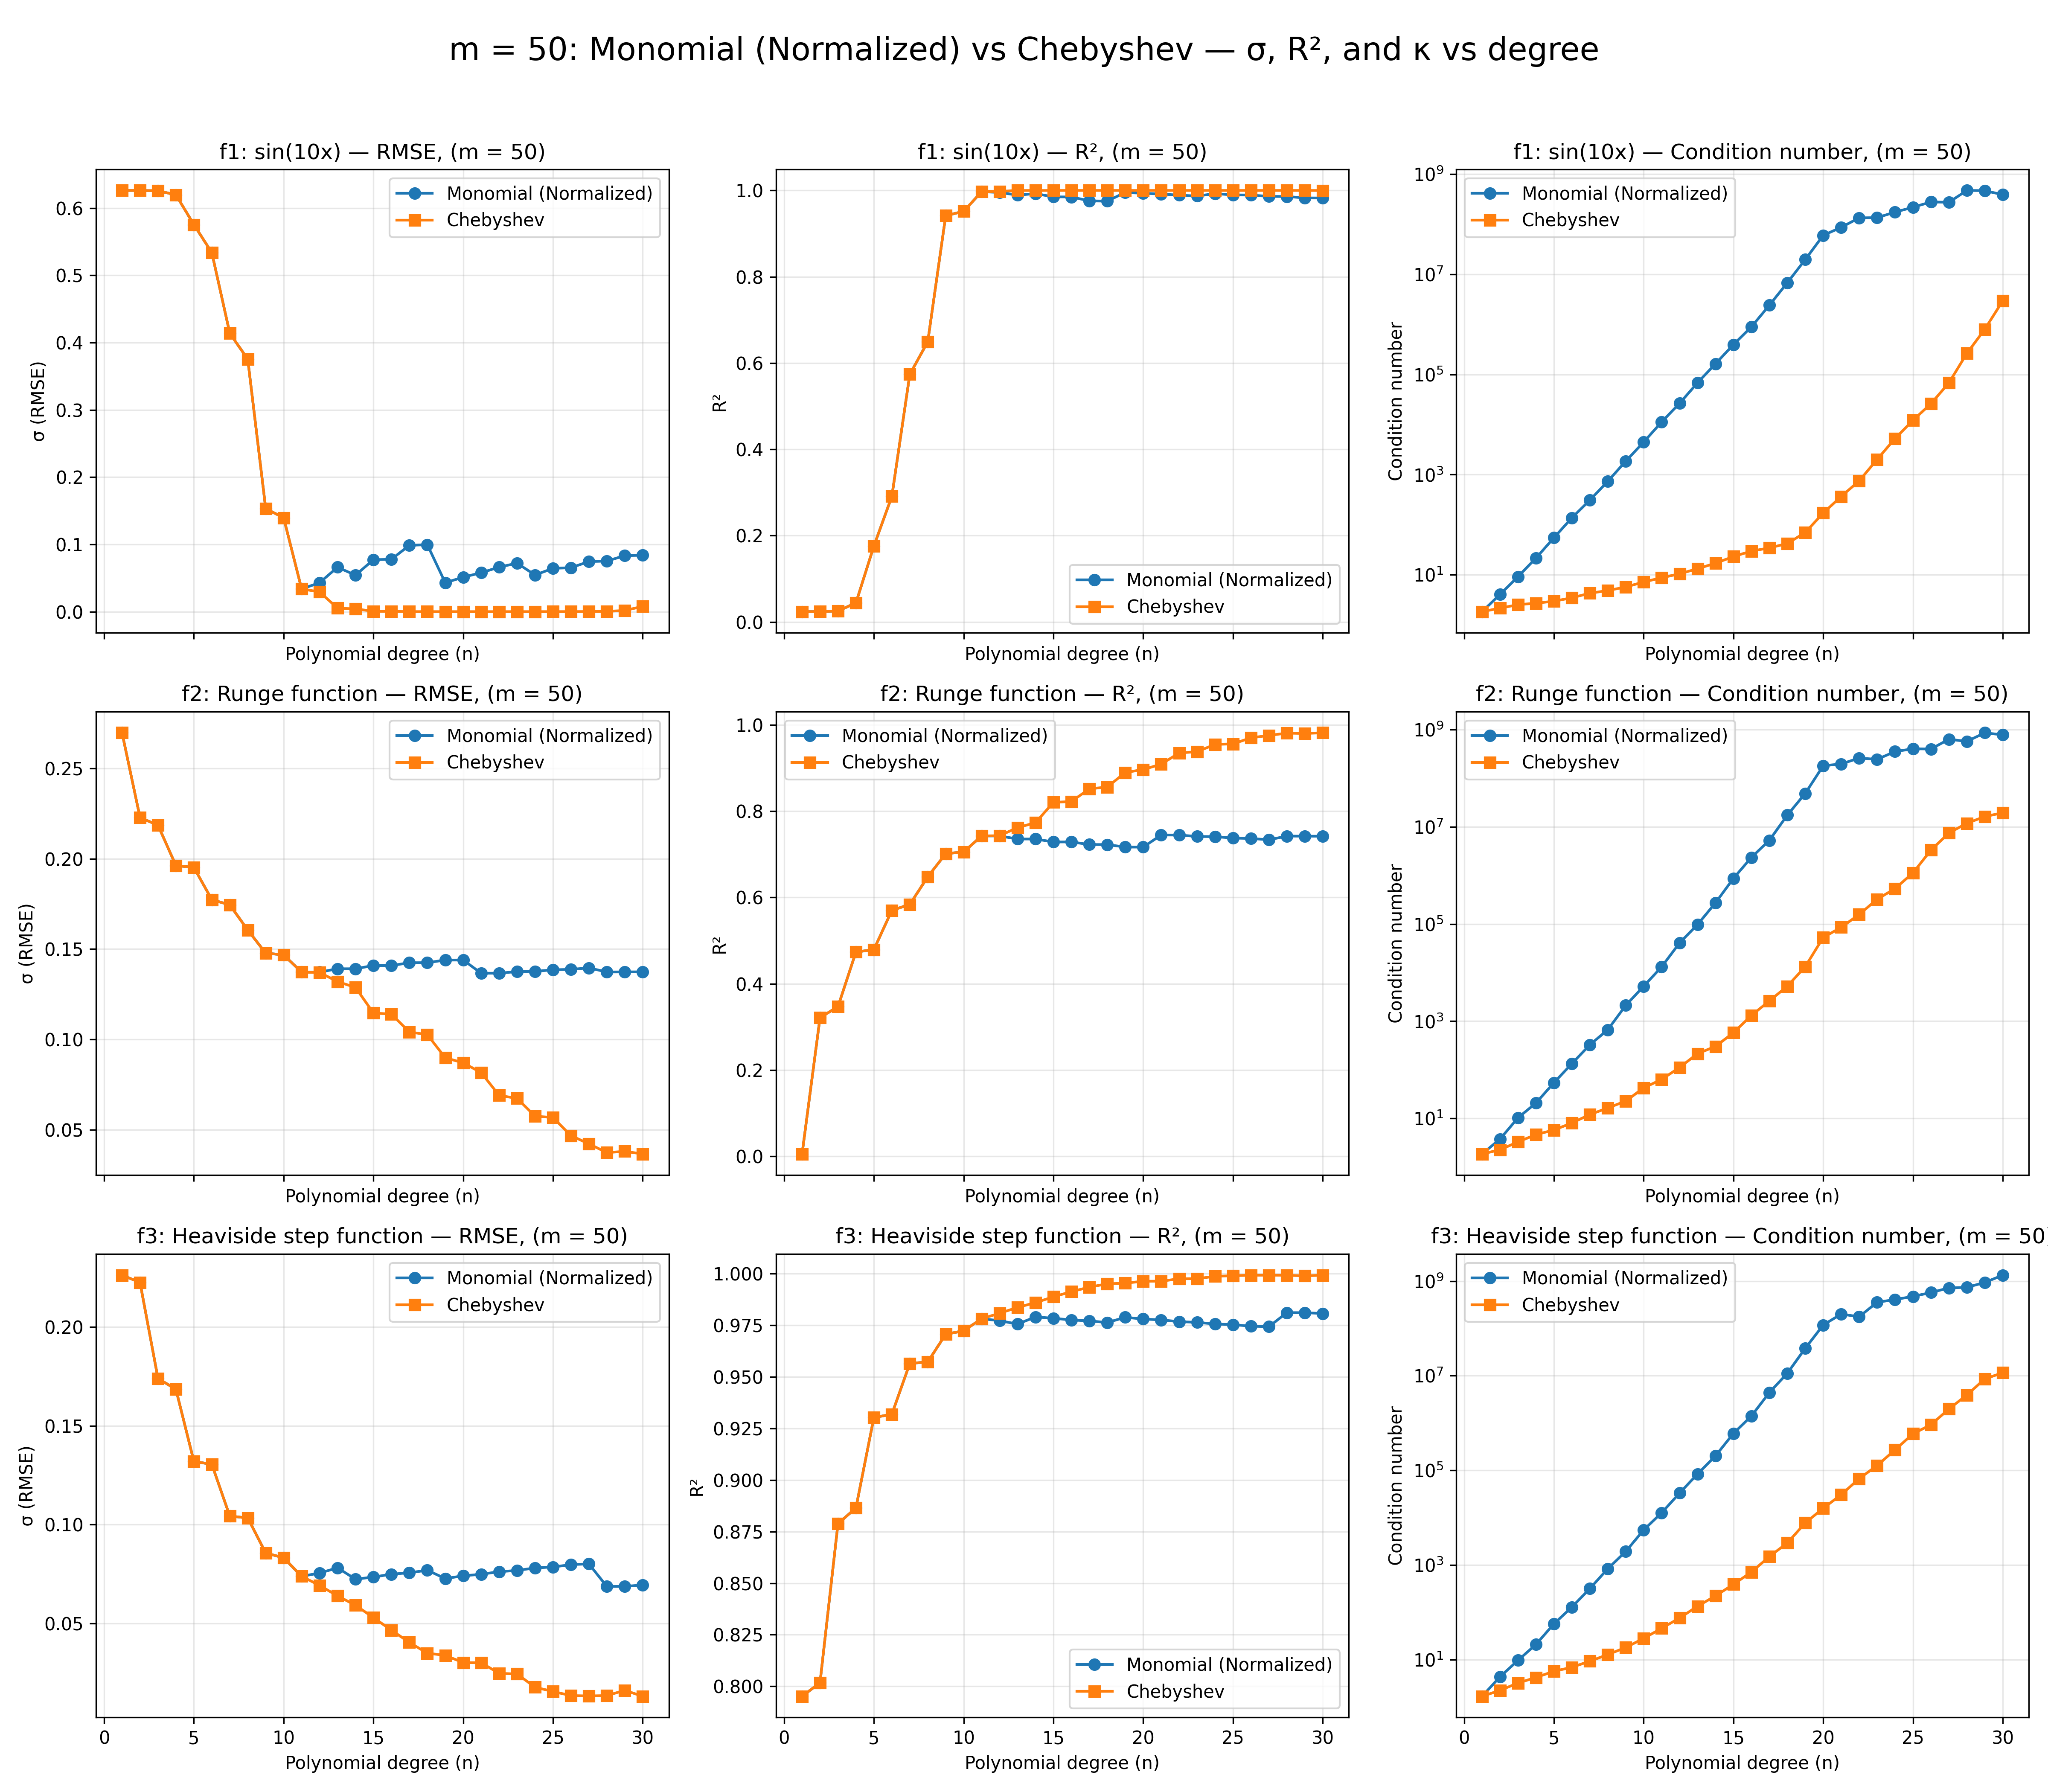
\includegraphics[width=\textwidth]{fig/results_m50.png}
    \caption{Results for $m=50$. Standard deviation $\sigma$ and $R^2$ vs.\ polynomial degree $n$.}
    \label{fig:50}
\end{figure}


\begin{figure}[h!]
    \centering
    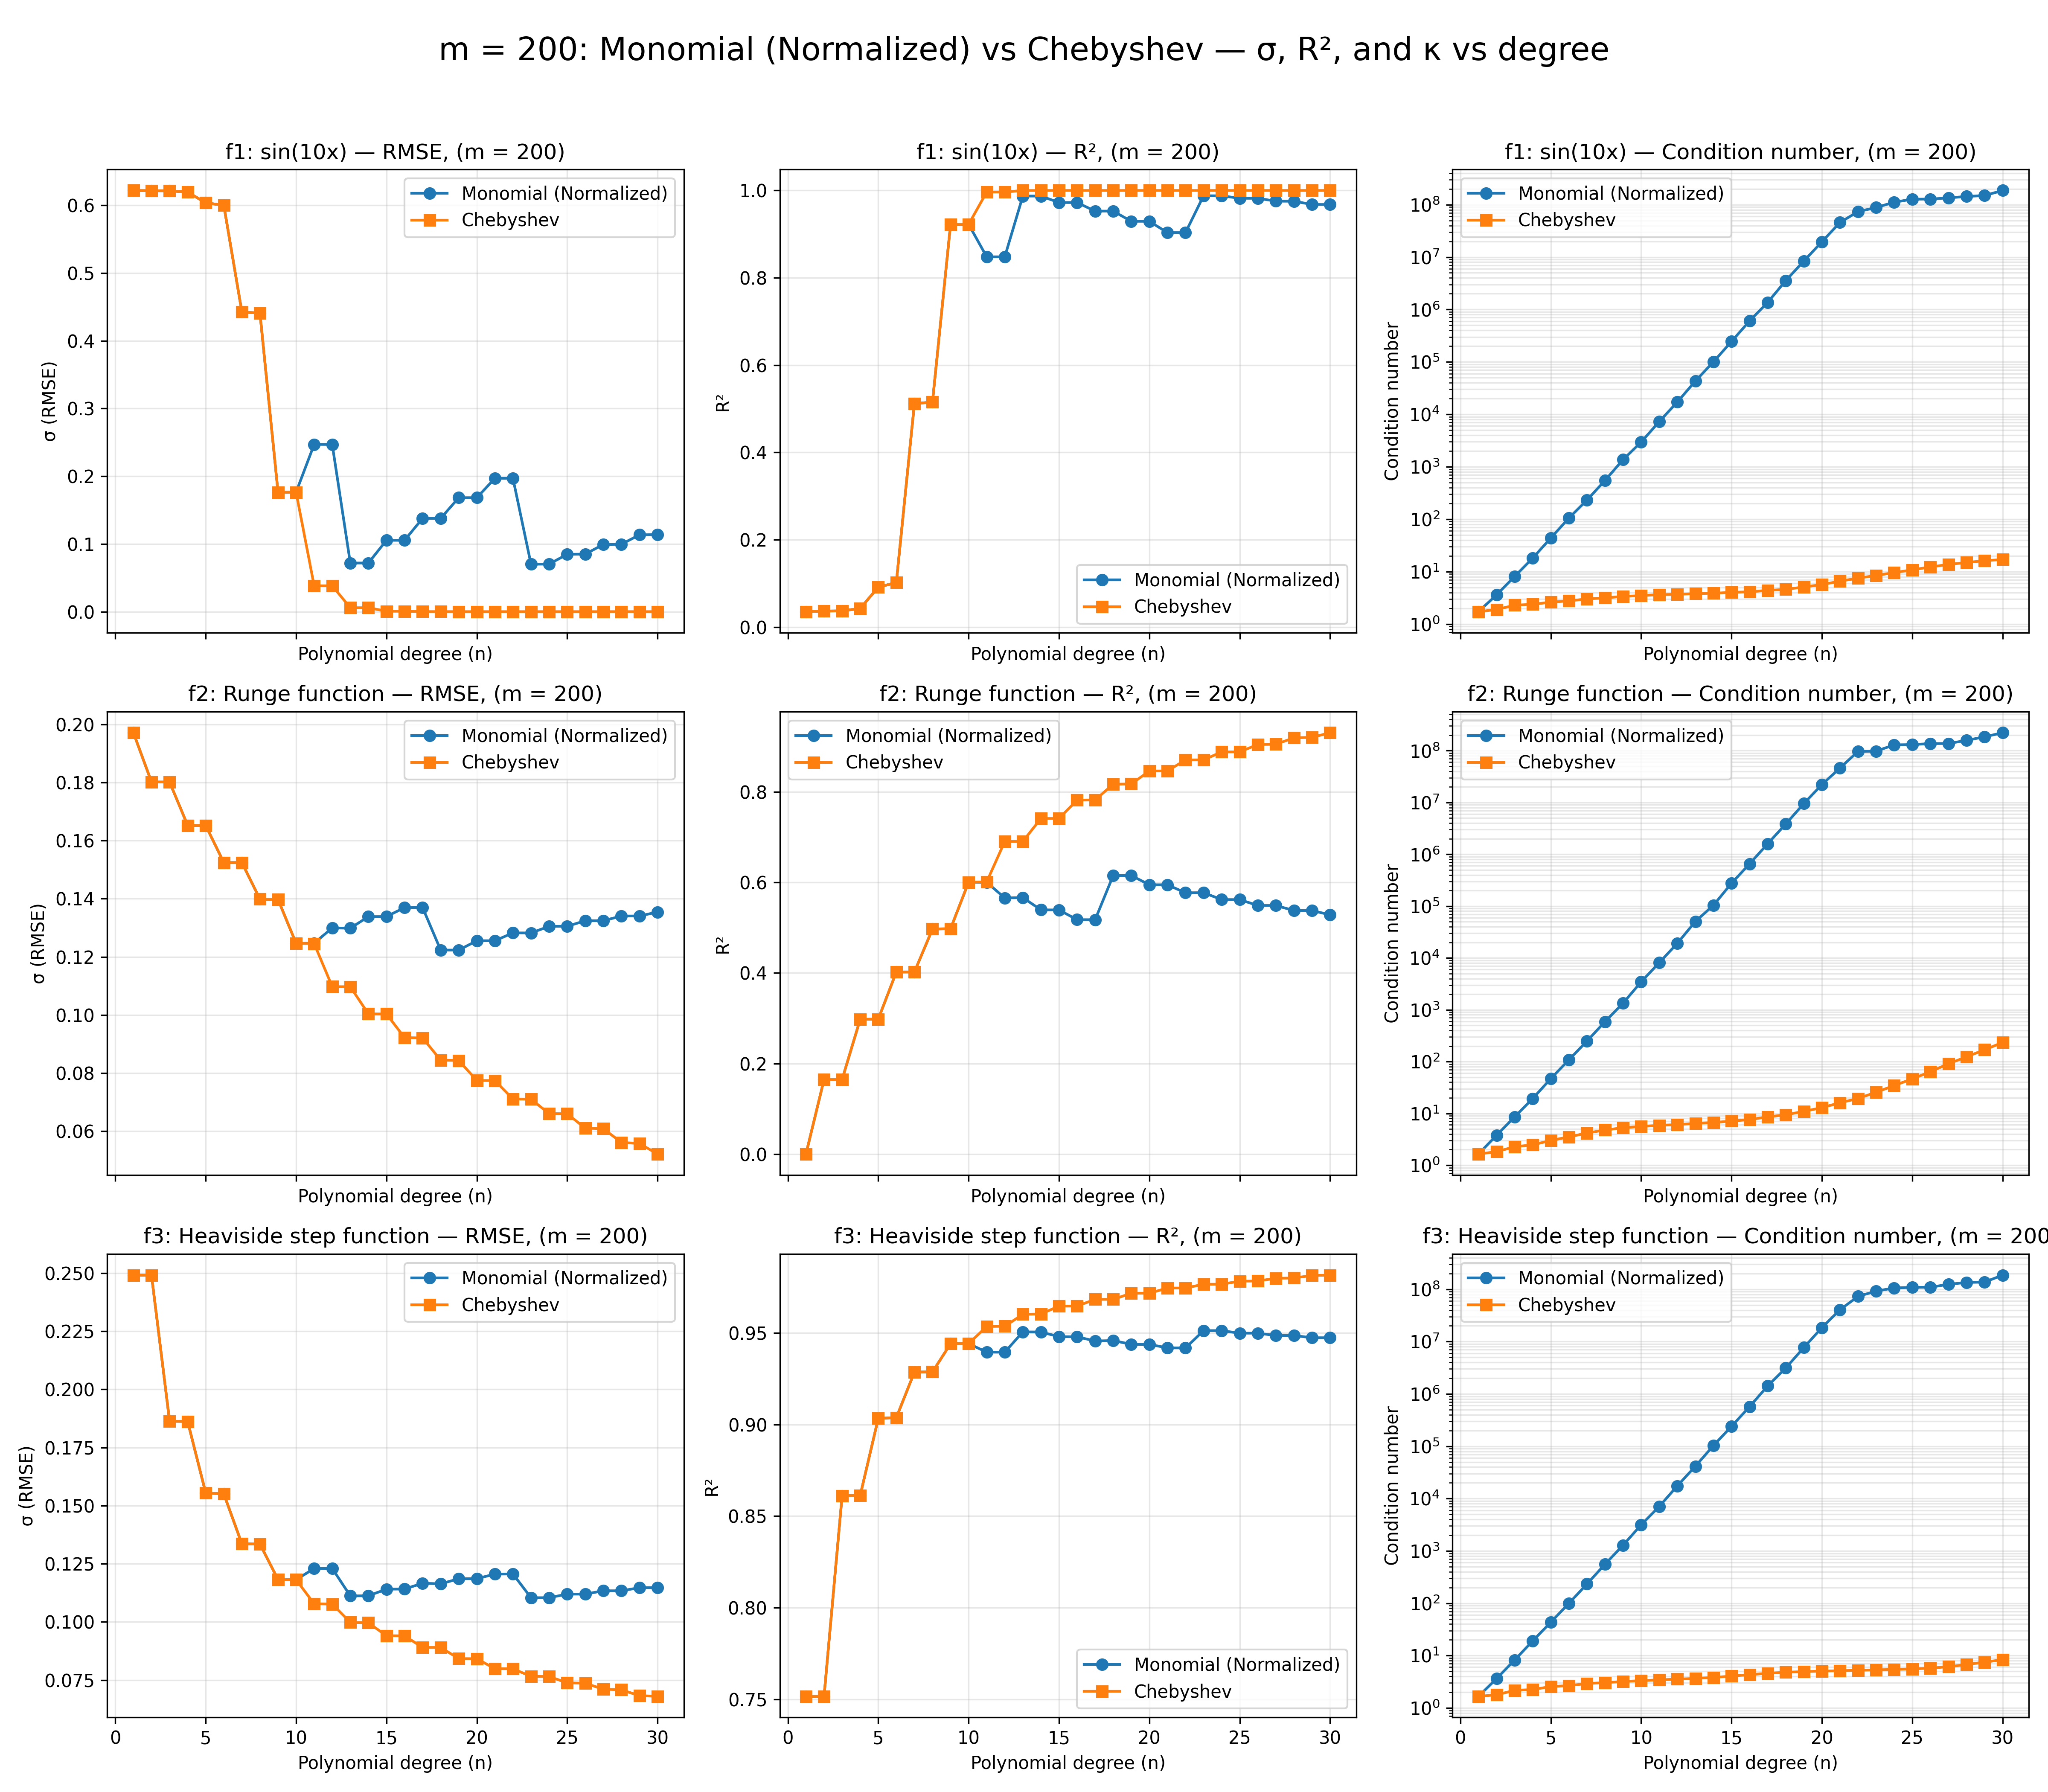
\includegraphics[width=\textwidth]{fig/results_m200.png}
    \caption{Results for $m=200$. Standard deviation $\sigma$ and $R^2$ vs.\ polynomial degree $n$.}
    \label{fig:200}
\end{figure}

\begin{figure}[h!]
    \centering
    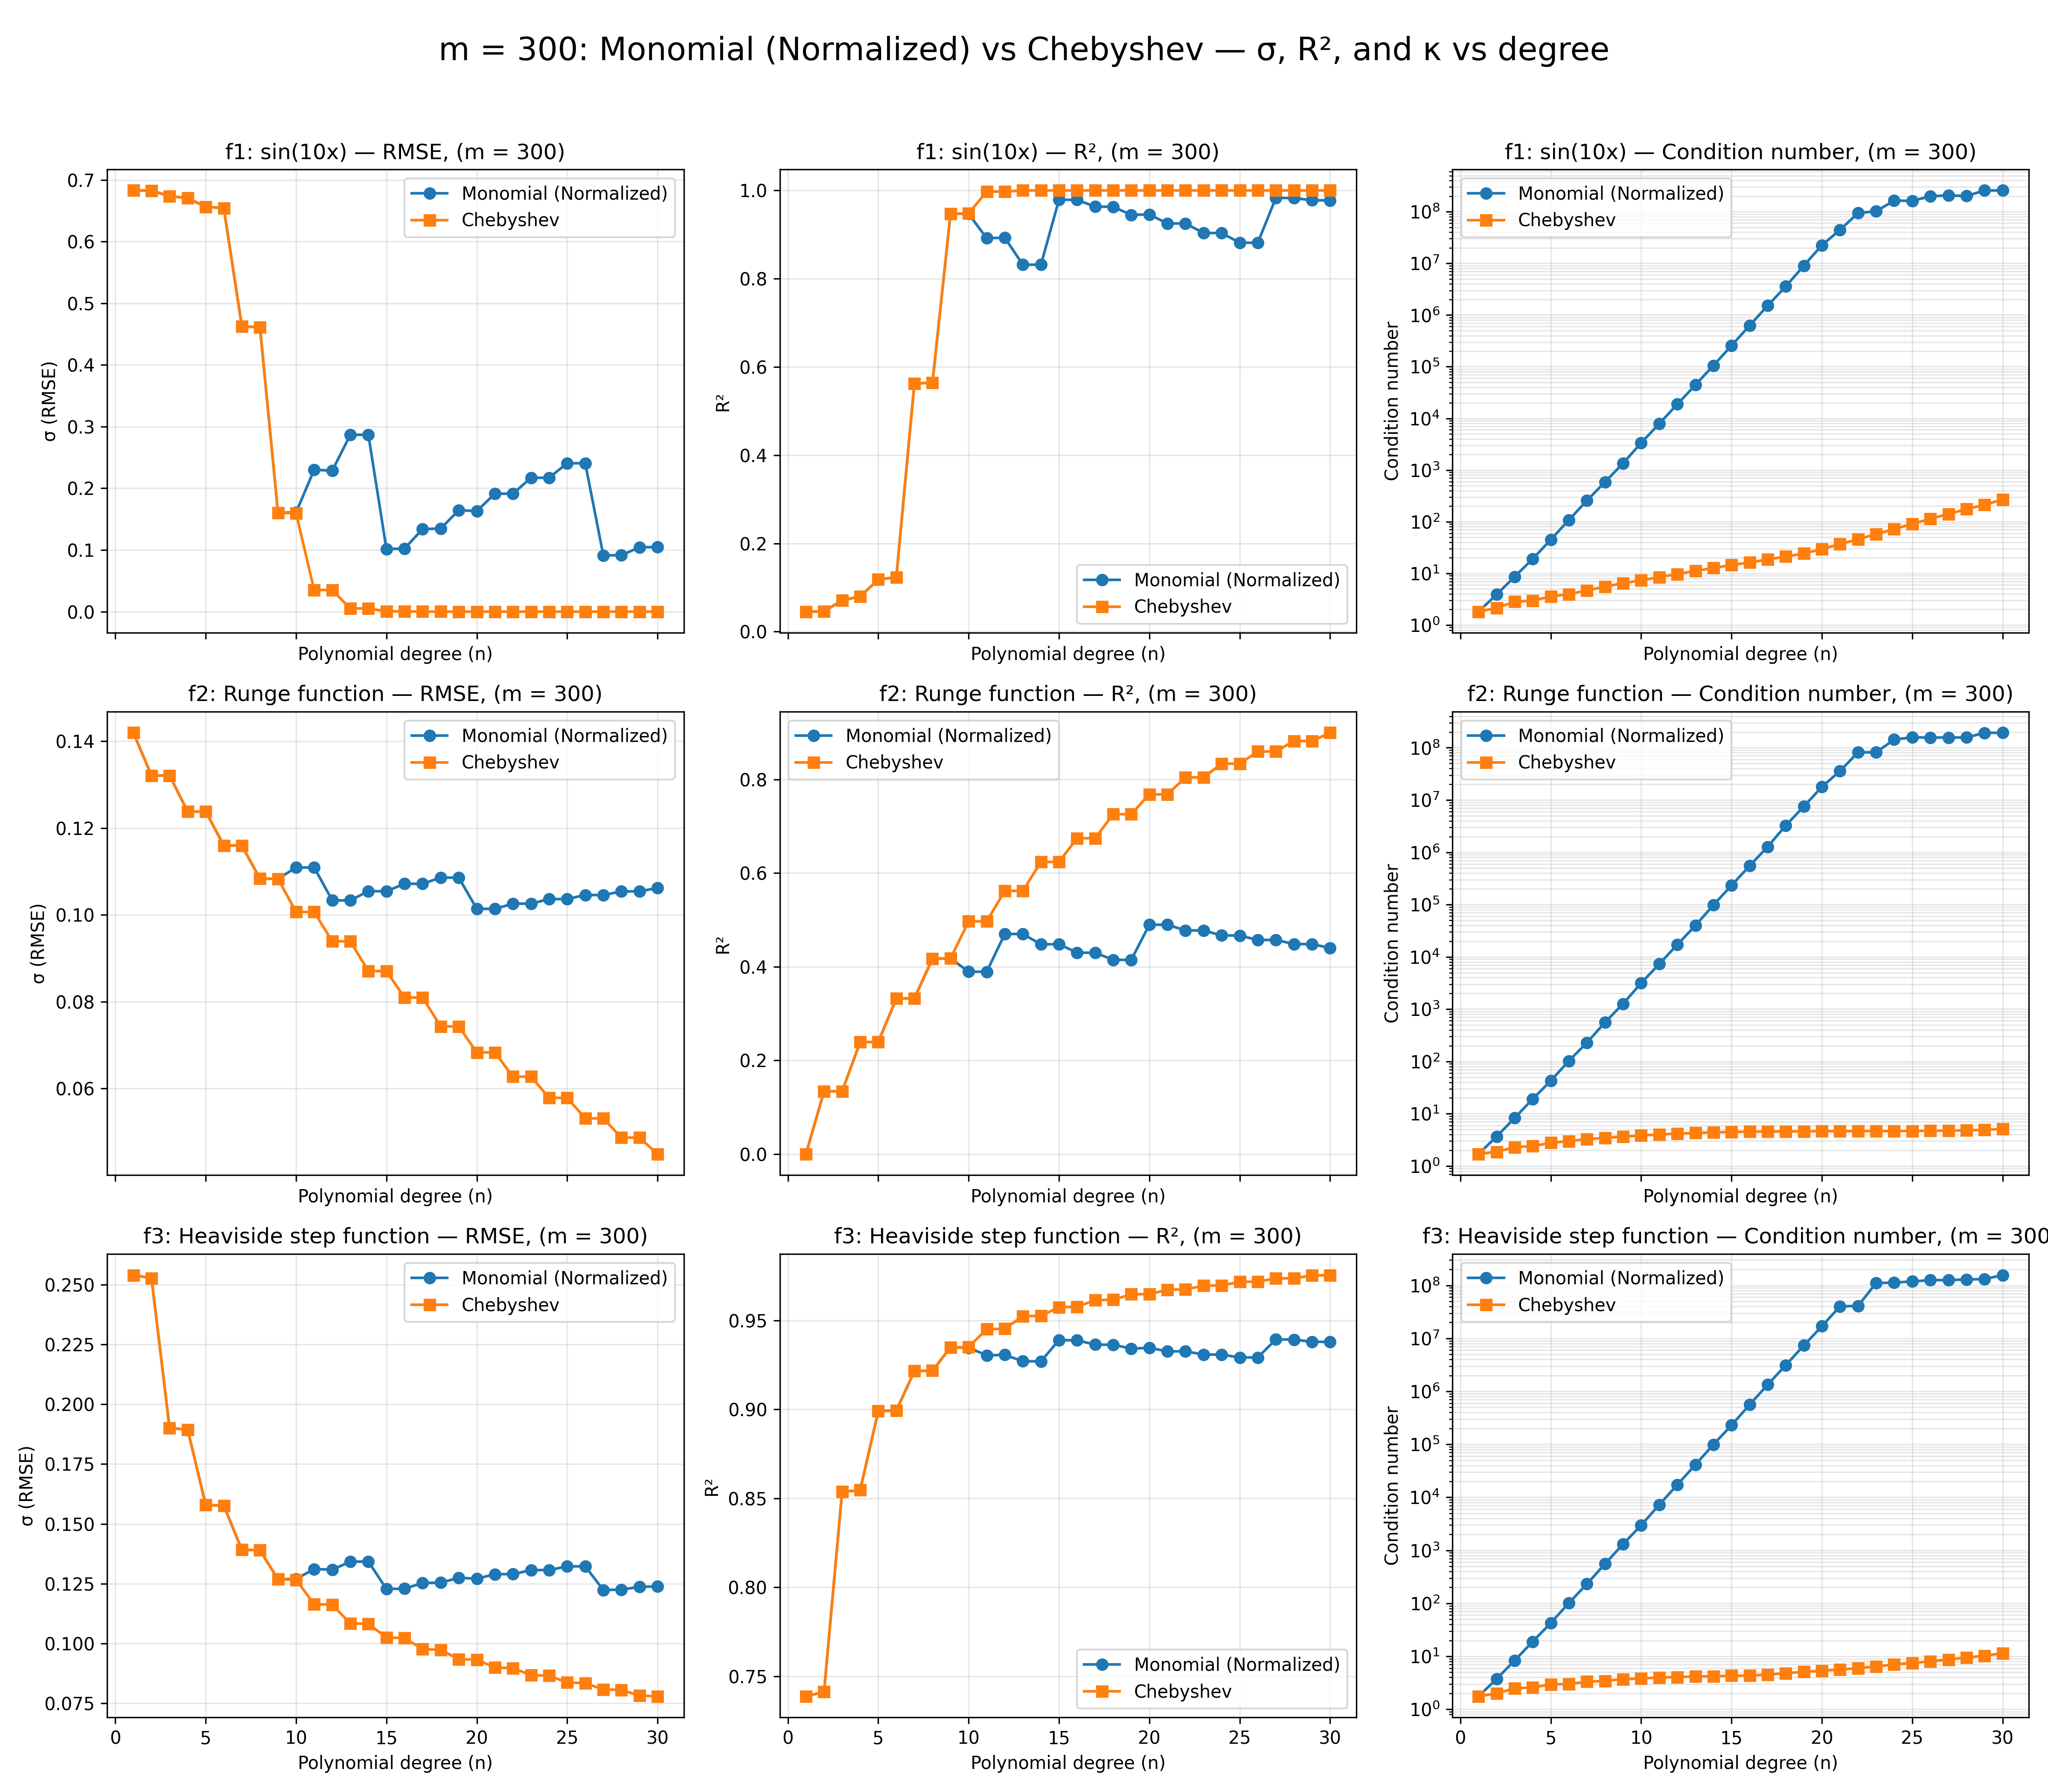
\includegraphics[width=\textwidth]{fig/results_m300.png}
    \caption{Results for $m=300$. Standard deviation $\sigma$ and $R^2$ vs.\ polynomial degree $n$.}
    \label{fig:300}
\end{figure}


\subsection*{Analysis and Discussion}
The results show clear differences between polynomial fitting with monomial and Chebyshev bases. For smooth functions such as $\sin(10x)$, both bases achieve low RMSE and high $R^2$ at moderate polynomial degree. However, as the degree n increases, the monomial basis quickly becomes unstable: the condition number of its Vandermonde matrix grows exponentially, leading to numerical errors and poor fits despite high model complexity. In contrast, Chebyshev polynomials maintain stability, keeping the condition number much smaller and producing consistent improvements in accuracy up to higher degrees.

The Runge function $1/(1+25x^2)$ highlights the classical Runge’s phenomenon: monomials show large oscillations at the interval boundaries, whereas Chebyshev basis reduces these oscillations and achieves lower error. For the step function, neither basis performs well due to the discontinuity, but Chebyshev still provides a more controlled approximation. Increasing the sample size m improves results for both methods, but it does not resolve the instability of monomials at high degrees. Overall, the experiments demonstrate that basis choice is crucial: while monomials suffice at low degree, Chebyshev polynomials are far more reliable for higher-degree approximations.


\clearpage

\section*{Exercise 2: Understanding Linear Regression}

\subsection*{Problem Statement}
Minimize the loss function:
\[
\min_{\theta \in \mathbb{R}^{n+1}} \sum_{i=1}^m r_i^2(\theta) w_i, \quad w_i > 0, \quad r_i(\theta) = y_i - M(x_i; \theta),
\]
where \( M(x; \theta) = \sum_{j=0}^n \theta_j e_j(x) \), \( n \ll m \).

\begin{enumerate}
    \item Show that the loss function can be expressed in the form of \( \| A \theta - y \|^2 \) for an appropriate diagonal matrix \( D \). Present \( A \), \( D \), and \( y \).
    \item Derive the normal equation by setting the gradient with respect to \( \theta \) equal to zero.
    \item Compute the Hessian matrix of the loss function. What can we conclude about the convexity based on the Hessian matrix and the uniqueness of the solution?
    \item (Optional) Can you give a condition on \( A \) such that the solution is unique?
    \item (Optional) How does the Tikhonov regularization work in the above formulation?
\end{enumerate}

\subsection*{Solution}

\subsubsection*{(1) Expression of the Loss Function}
The loss function is:
\[
L(\theta) = \sum_{i=1}^m w_i r_i^2(\theta), \quad r_i(\theta) = y_i - M(x_i; \theta).
\]
In matrix form: 
\( A \) is the \( m \times (n+1) \) design matrix with \( A_{i,j} = e_j(x_i) \) (Vandermonde matrix for monomials),  \( y = [y_1, \ldots, y_m]^T \), 
\( D = \text{diag}(w_1, \ldots, w_m) \).
Thus:
\[
L(\theta) = (y - A \theta)^T D (y - A \theta) = \| \sqrt{D} (A \theta - y) \|^2.
\]

\subsubsection*{(2) Normal Equation}
The gradient is:
\[
\nabla_\theta L = -2 A^T D (y - A \theta).
\]
Setting it to zero:
\[
A^T D A \theta = A^T D y.
\]
The solution is \( \theta^* = (A^T D A)^{-1} A^T D y \) if invertible.

%If $A$ has full column rank, $H \succ 0$ and the problem is strictly convex with a unique minimizer.  With Tikhonov regularization,
%\[
%(A^TDA + \lambda I)\theta = A^T Dy,
%\]
%which improves conditioning and guarantees invertibility.

\subsubsection*{(3) Hessian and Convexity}
The Hessian is:
\[
H = 2 A^T D A.
\]

\textbf{Convexity}: \( z^T H z = 2 (A z)^T D (A z) \geq 0 \) (positive semi-definite). If \( A \) is full rank and \( D \) is positive definite, \( H \) is positive definite, making \( L(\theta) \) strictly convex.

\textbf{Uniqueness}: Unique if \( H \) is invertible, i.e., \( A \) has full column rank.

\subsubsection*{(4) Condition for Uniqueness}
\( A \) must have full column rank (\( \text{rank}(A) = n+1 \)), ensured by distinct \( x_i \) and \( m > n \).

\subsubsection*{(5) Tikhonov Regularization}
Add penalty:
\[
L_{\text{reg}}(\theta) = (y - A \theta)^T D (y - A \theta) + \lambda \| \theta \|^2.
\]
Gradient:
\[
\nabla_\theta L_{\text{reg}} = -2 A^T D (y - A \theta) + 2 \lambda \theta = 0,
\]
yielding:
\[
(A^T D A + \lambda I) \theta = A^T D y.
\]
This ensures invertibility and reduces \( \theta \) magnitude, improving stability.

\clearpage

\section*{Exercise 3: Extension to Nonlinear Regression}

\subsection*{Problem Statement}
Minimize:
\[
\min_{\theta} L(\theta) = \sum_{i=1}^m \rho(r_i(\theta)), \quad r_i(\theta) = y_i - M(x_i; \theta).
\]
Use iterative methods with monomial basis for:
\begin{enumerate}
    \item Huber loss.
    \item \( l^p \), \( p = 1.5 \).
\end{enumerate}
Report max error \( \max_{j=1}^{1000} | \Gamma(x_j) - M(x_j; \theta) | \) where \( x_j = a + j (b - a) / 1000 \), \( m = 100 \).

\subsection*{Solution}
\begin{lstlisting}
import jax
import jax.numpy as jnp
import jax.random as random
import matplotlib.pyplot as plt
import csv
from dataclasses import dataclass

# Datasets (Gamma functions)
def f1(x):  # sin(10x) on [-1, 1]
    return jnp.sin(10.0 * x)

def f2(x):  # Runge function on [-5, 5]
    return 1.0 / (1.0 + 25.0 * x**2)

def f3(x):  # Step function on [-2, 2]: 1 in [0,2], else 0
    return jnp.where((x >= 0.0) & (x <= 2.0), 1.0, 0.0)

@dataclass
class Dataset:
    f: callable
    a: float
    b: float
    name: str

DATASETS = [
    Dataset(f=f1, a=-1.0, b= 1.0, name="sin(10x)"),
    Dataset(f=f2, a=-5.0, b= 5.0, name="Runge function"),
    Dataset(f=f3, a=-2.0, b= 2.0, name="Heaviside step function"),
]

# Losses
def huber_loss(r, delta=1.0):
    # 0.5 r^2 for |r|<=delta, delta(|r| - 0.5 delta) otherwise
    absr = jnp.abs(r)
    quad = 0.5 * r**2
    lin = delta * (absr - 0.5 * delta)
    return jnp.where(absr <= delta, quad, lin)

def lp_loss(r, p=1.5):
    return jnp.abs(r)**p

# Names for plotting/CSV
LOSS_SPECS = [
    ("huber", lambda r: huber_loss(r, delta=1.0)),
    ("lp",    lambda r: lp_loss(r, p=1.5)),
]

# Utilities
def normalize_to_unit_interval(x, a, b):
    return 2.0 * (x - a) / (b - a) - 1.0

def vandermonde(x_norm, degree):
    return jnp.vander(x_norm, degree + 1, increasing=True)

def initial_theta(A, y):
    try:
        return jnp.linalg.lstsq(A, y, rcond=None)[0]
    except AttributeError:
        return jnp.linalg.pinv(A) @ y

# IRLS core (weights per assignment: w = rho(r) / r^2)
def irls(A, y, rho_fn, max_iter=1000, tol=1e-8, eps=1e-8):
    """
    Solve min sum_i rho(r_i) via IRLS:
      - r = y - A @ theta
      - w_i = rho(r_i) / (r_i^2 + eps)
      - Solve weighted LS: min_theta || diag(sqrt(w)) (y - A theta) ||^2
    """
    theta = initial_theta(A, y)
    for _ in range(max_iter):
        r = y - A @ theta
        rho_val = rho_fn(r)
        w = rho_val / (r**2 + eps)
        # Weighted least squares: minimize || W^(1/2) (y - A theta) ||_2
        # Equivalent normal eq: (A^T W A) theta = A^T W y
        # We'll form W*A and W*y via diag weights:
        sqrtw = jnp.sqrt(w)
        Aw = A * sqrtw[:, None]
        yw = y * sqrtw
        theta_new = jnp.linalg.pinv(Aw) @ yw

        if jnp.linalg.norm(theta_new - theta) < tol:
            return theta_new
        theta = theta_new
    return theta  # reached max_iter

# Experiment configuration
m = 100
degrees = list(range(1, 31))  # 1..30
num_test = 1000
key = random.PRNGKey(0)

# Run experiments
results = []  # rows: (dataset, loss, degree, max_error)

for (loss_name, rho_fn) in LOSS_SPECS:
    for ds in DATASETS:
        a, b, f, name = ds.a, ds.b, ds.f, ds.name

        # Training data
        key, subkey = random.split(key)
        
        x_train = jnp.linspace(a, b, m)
        y_train = f(x_train)

        # Normalize x to [-1,1] for stability; build test grid too
        x_train_norm = normalize_to_unit_interval(x_train, a, b)
        
        #x_test = jnp.linspace(a, b, num_test)
        x_test = random.uniform(subkey, shape=(m,), minval=a, maxval=b)
        x_test_norm = normalize_to_unit_interval(x_test, a, b)
        y_test_true = f(x_test)

        # Sweep degrees
        for n in degrees:
            # Design matrices
            A = vandermonde(x_train_norm, n)
            A_test = vandermonde(x_test_norm, n)

            # Initial LS (warm start), then IRLS
            theta0 = initial_theta(A, y_train)
            # IRLS using the assignment's weight rule
            theta = irls(A, y_train, rho_fn=rho_fn, max_iter=1000, tol=1e-8, eps=1e-8)

            # Evaluate required metric
            y_pred = A_test @ theta
            err_max = jnp.max(jnp.abs(y_test_true - y_pred))
            results.append((name, loss_name, int(n), float(err_max)))

            # Console progress
            print(f"{name:26s} | loss={loss_name:5s} | n={n:2d} | max_err={float(err_max):.6e}")


# Save CSV of results
csv_path = "exercise3_results.csv"
with open(csv_path, "w", newline="") as f:
    writer = csv.writer(f)
    writer.writerow(["dataset", "loss", "degree_n", "max_error"])
    writer.writerows(results)
print(f"\nSaved results to {csv_path}")

# Plot error vs degree
import pandas as pd

df = pd.DataFrame(results, columns=["dataset", "loss", "degree_n", "max_error"])
for ds in DATASETS:
    sub = df[df["dataset"] == ds.name].copy()
    # Pivot to have columns per loss
    pivot = sub.pivot(index="degree_n", columns="loss", values="max_error").sort_index()

    plt.figure(figsize=(5, 4))
    if "huber" in pivot.columns:
        plt.plot(pivot.index.values, pivot["huber"].values, marker="o", label="Huber")
    if "lp" in pivot.columns:
        plt.plot(pivot.index.values, pivot["lp"].values, marker="s", label="L^1.5")

    plt.title(f"Max Error vs Degree — {ds.name}")
    plt.xlabel("Polynomial degree n")
    plt.ylabel("Max error on 1000 test points")
    plt.grid(True, alpha=0.4)
    plt.legend()
    out_png = f"exercise3_error_vs_degree_{ds.name.replace(' ', '_').replace('(', '').replace(')', '')}.png"
    plt.tight_layout()
    plt.savefig(out_png, dpi=300)
    plt.close()
    print(f"Saved plot: {out_png}")
\end{lstlisting}


%Max error reported for each dataset and loss function.
\subsection*{Results}
\Cref{fig:comparison} and \Cref{fig:comparison(1)} compares Huber and $L^{1.5}$ losses at $n=10$ with uniformly spaced training points and with randomly sampled training points. As shown in \Cref{fig:error-vs-degree} and Table~\ref{tab:max-error}, the maximum error decreases with increasing polynomial degree for the smooth and oscillatory functions, while the discontinuous case remains difficult.

\begin{figure}[b!]
    \centering
    
    % ---- Left block ----
    \begin{minipage}{0.49\textwidth}
        \centering
        %\caption*{Huber loss}
        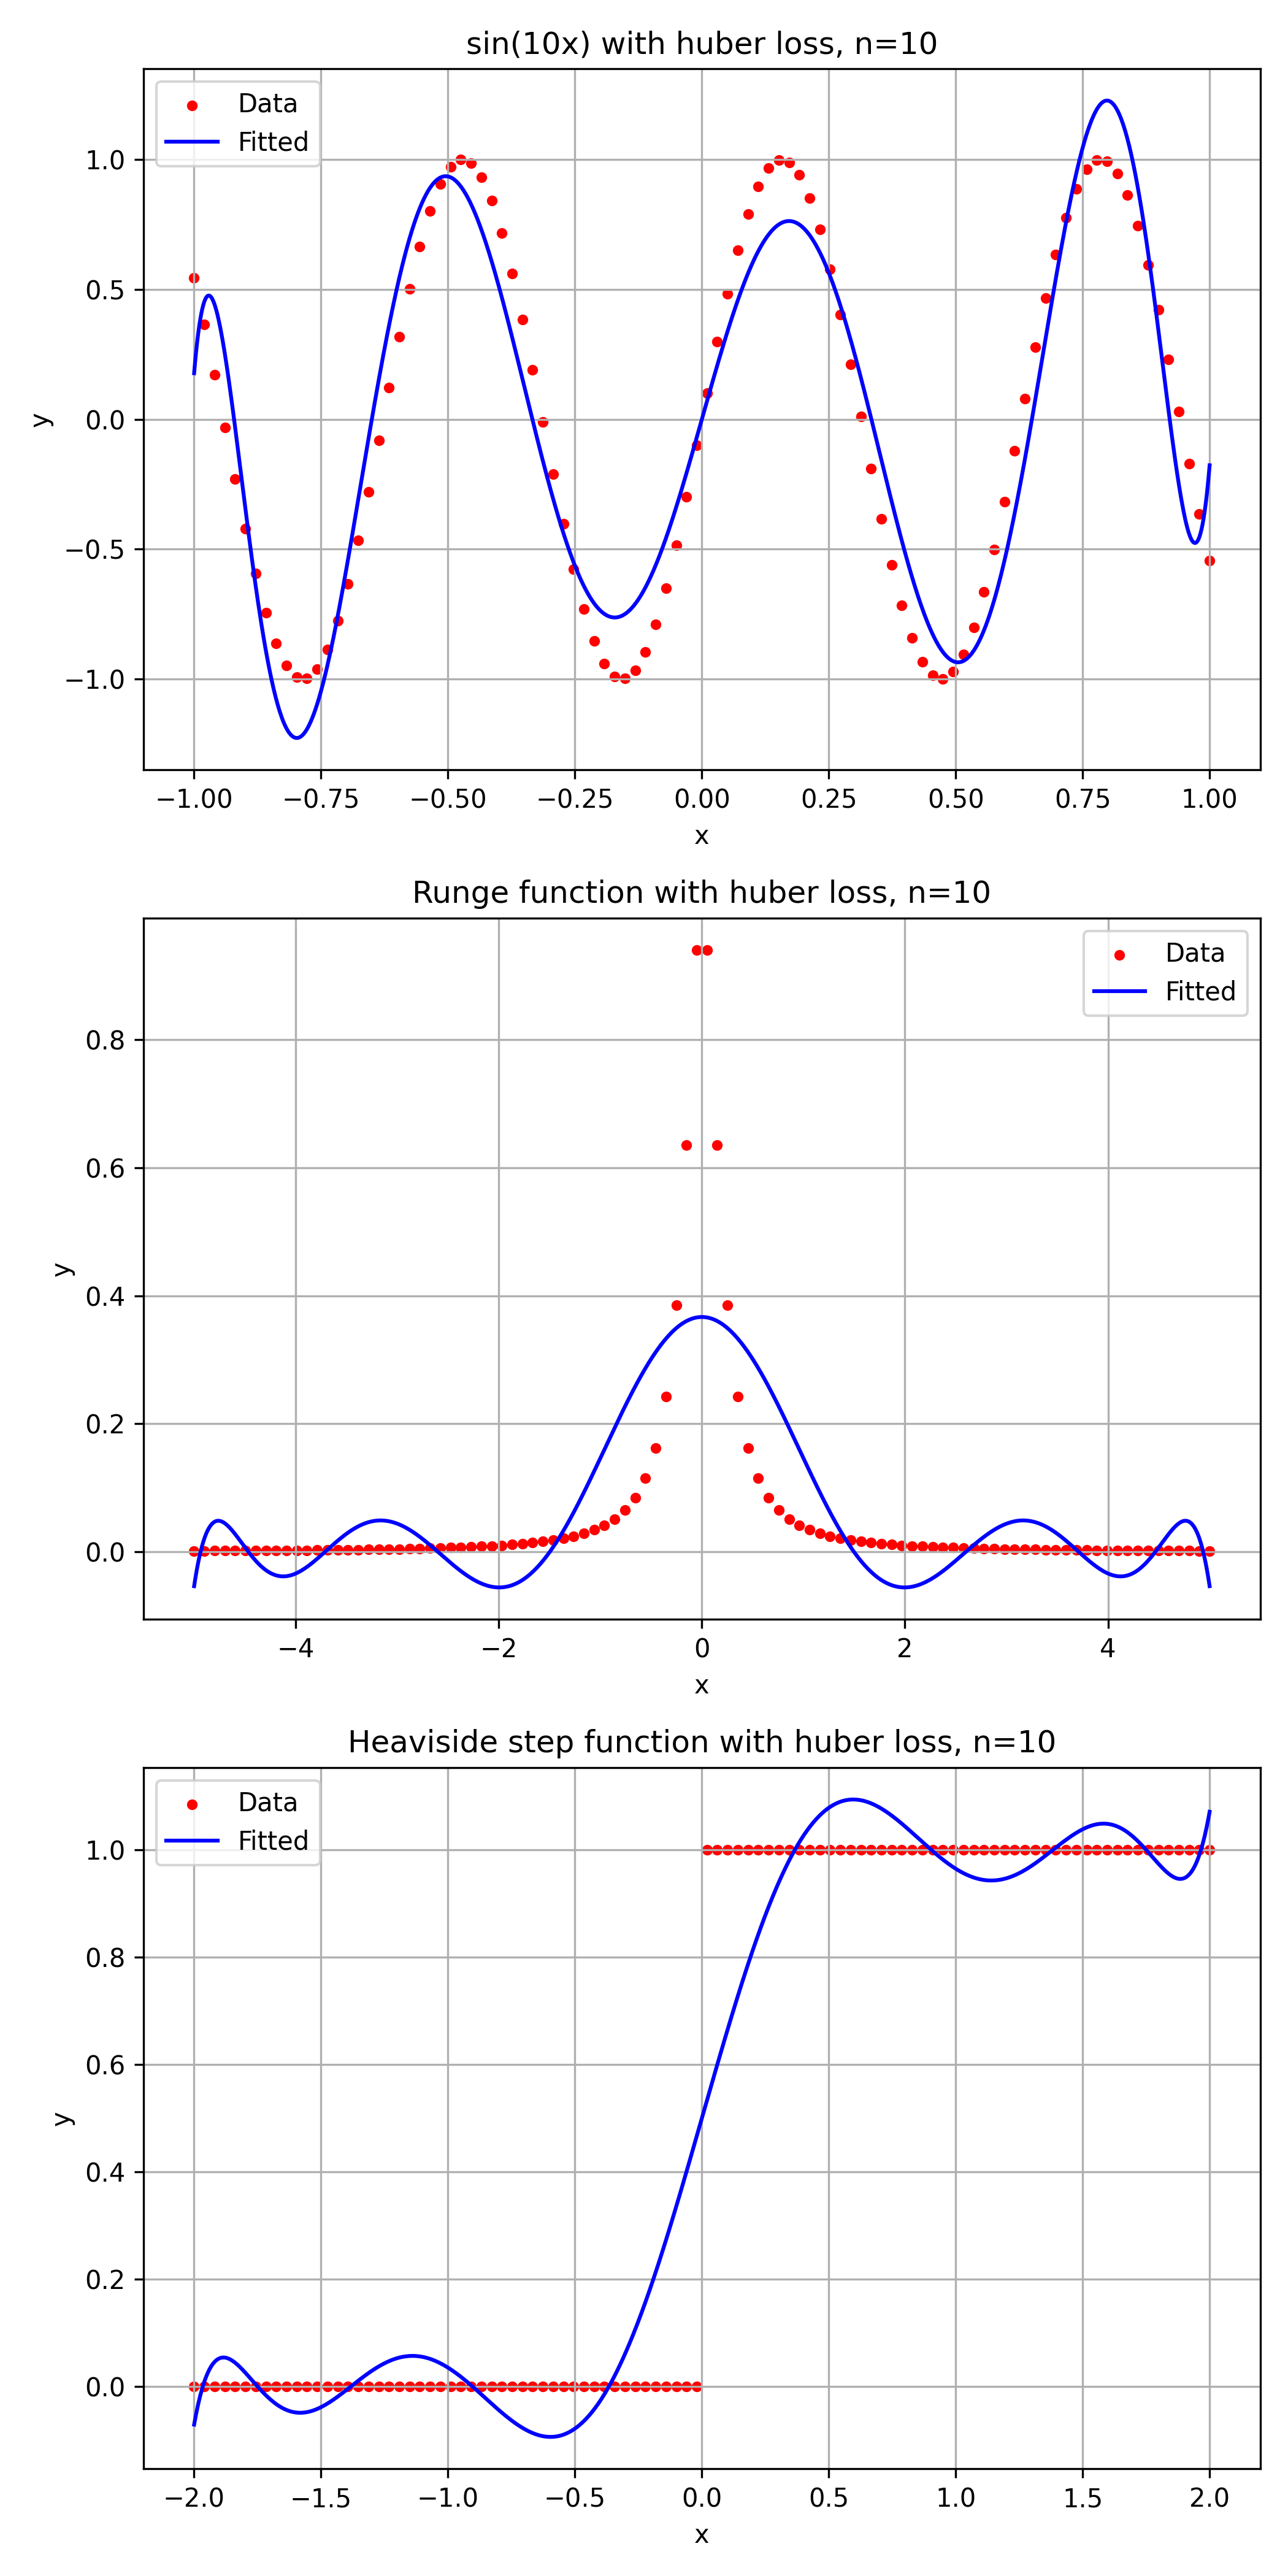
\includegraphics[width=\linewidth]{fig/compare_huber_loss.png}
    \end{minipage}
    \hfill
    % ---- Right block ----
    \begin{minipage}{0.49\textwidth}
        \centering
         %\caption*{\( l^p \)}
        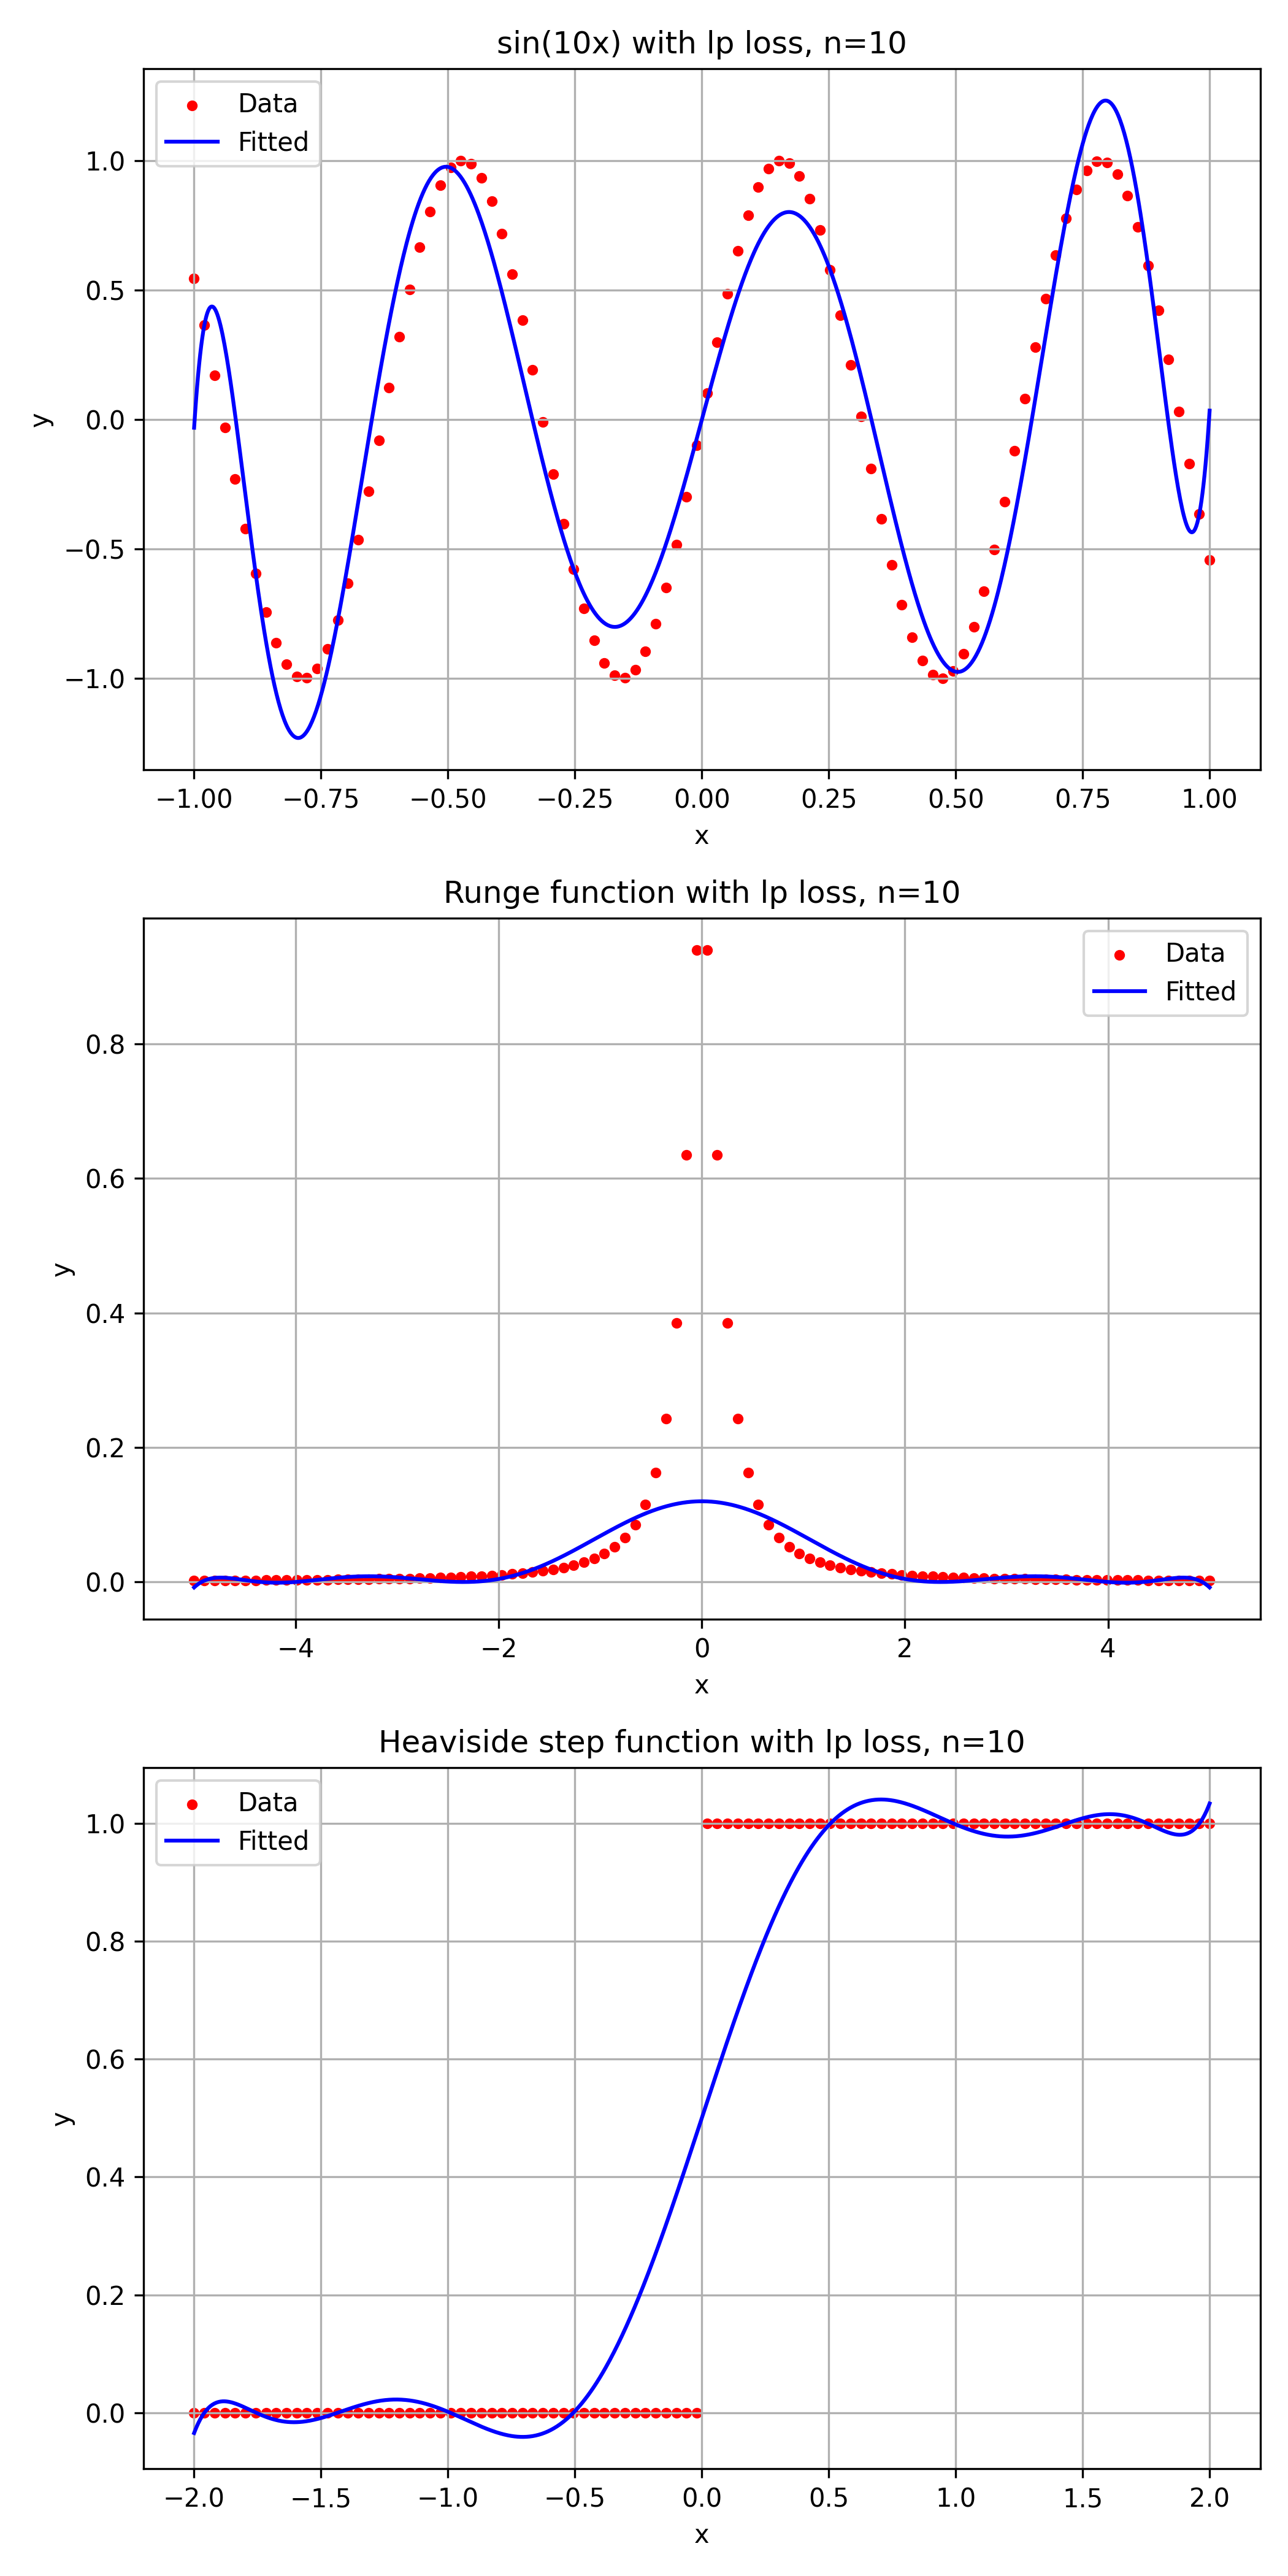
\includegraphics[width=\linewidth]{fig/compare_lp_loss.png}
        % local caption
    \end{minipage}

    % Global caption
    \caption{Comparison of Huber loss vs \( l^p \) with three functions ($n=10$, with uniformly spaced dataset).}
    \label{fig:comparison}
\end{figure}


\begin{figure}[b!]
    \centering
    
    % ---- Left block ----
    \begin{minipage}{0.49\textwidth}
        \centering
        %\caption*{Huber loss}
        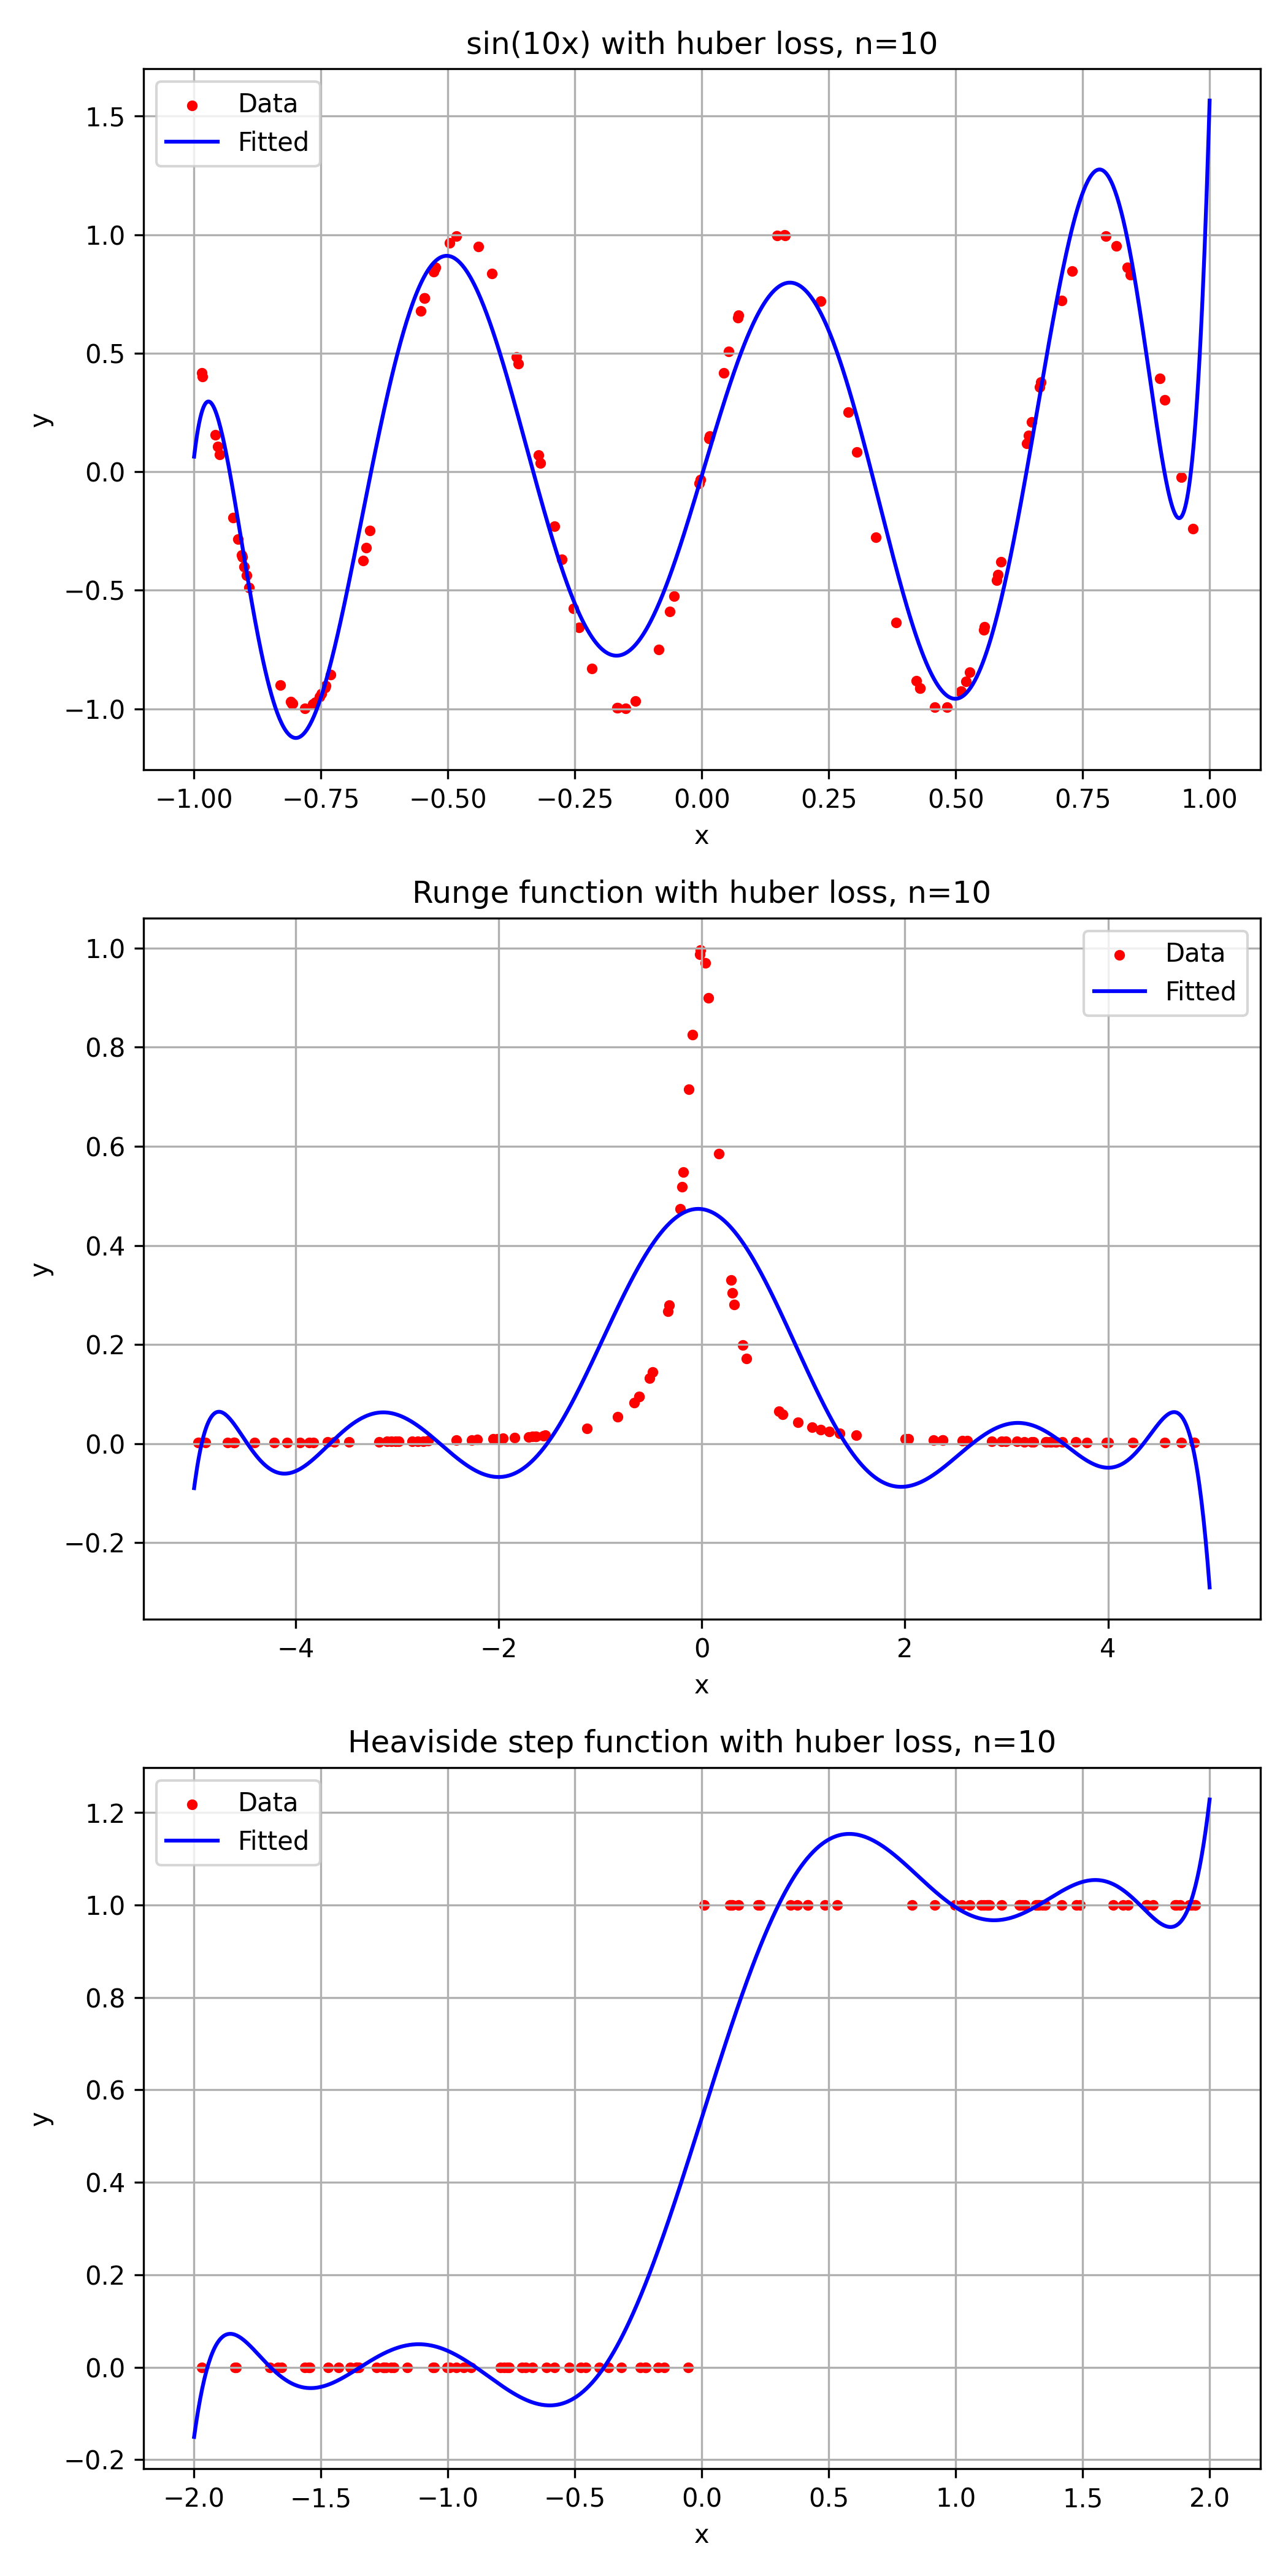
\includegraphics[width=\linewidth]{fig/compare_huber_loss (1).png}
    \end{minipage}
    \hfill
    % ---- Right block ----
    \begin{minipage}{0.49\textwidth}
        \centering
         %\caption*{\( l^p \)}
        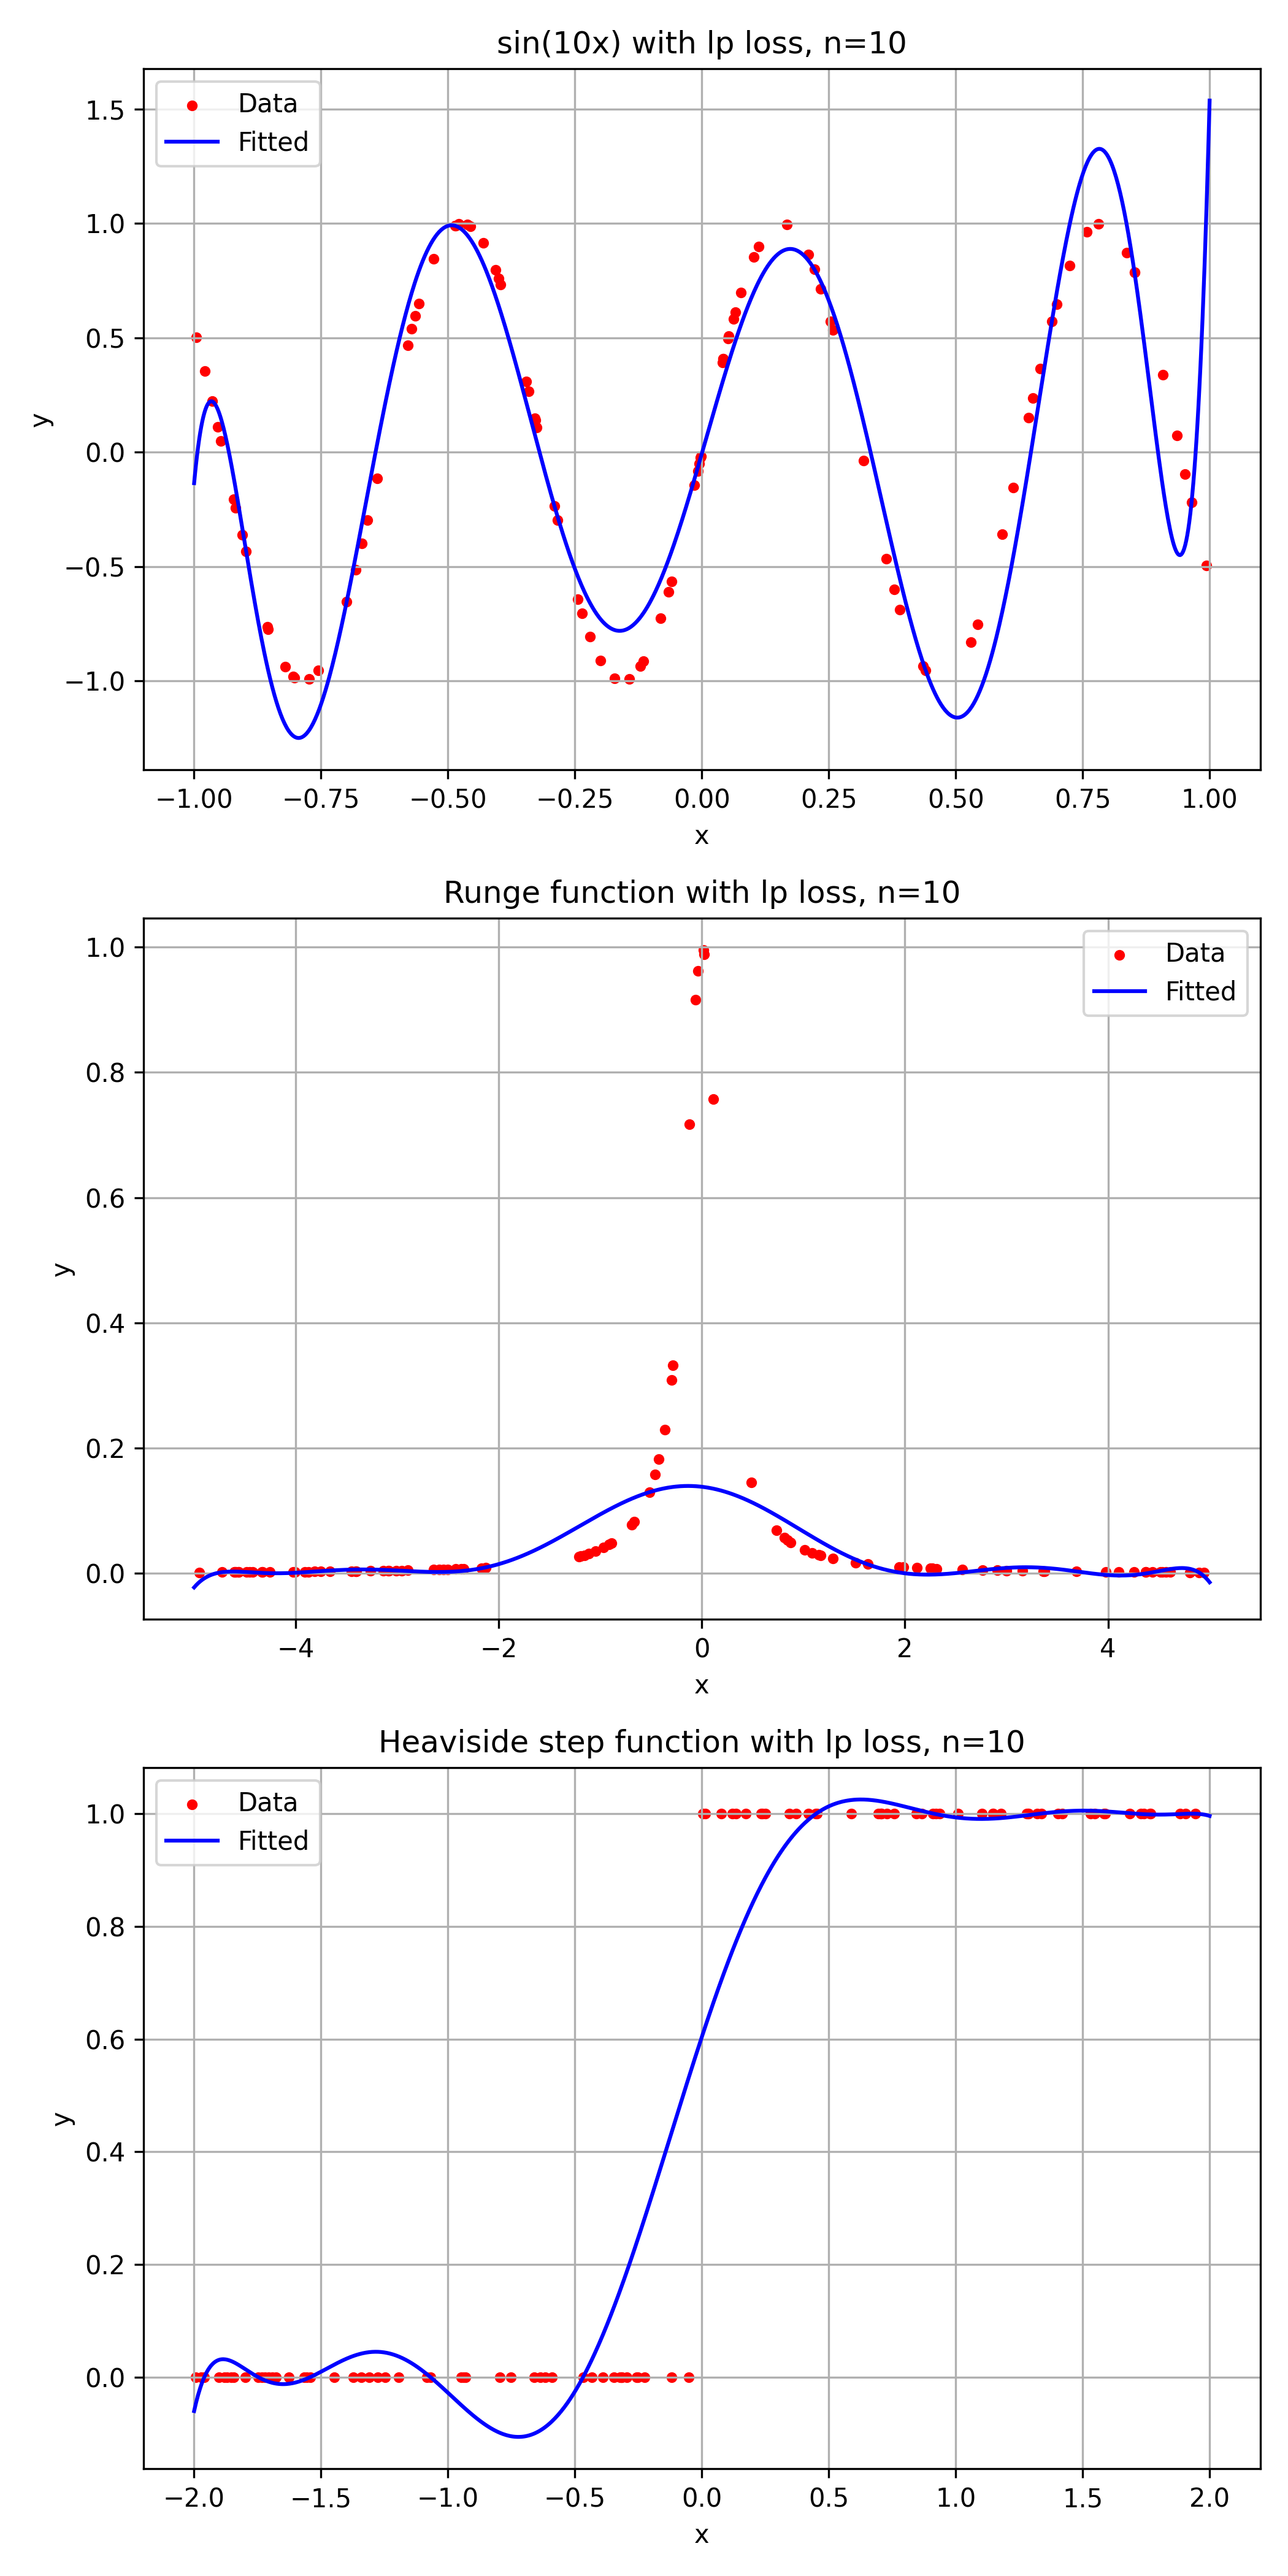
\includegraphics[width=\linewidth]{fig/compare_lp_loss (1).png}
        % local caption
    \end{minipage}

    % Global caption
    \caption{Comparison of Huber loss vs \( l^p \) with three functions ($n=10$, with randomly sampled training points).}
    \label{fig:comparison(1)}
\end{figure}

\begin{figure}[h!]
    \centering
    \begin{subfigure}[b]{0.49\linewidth}
        \centering
        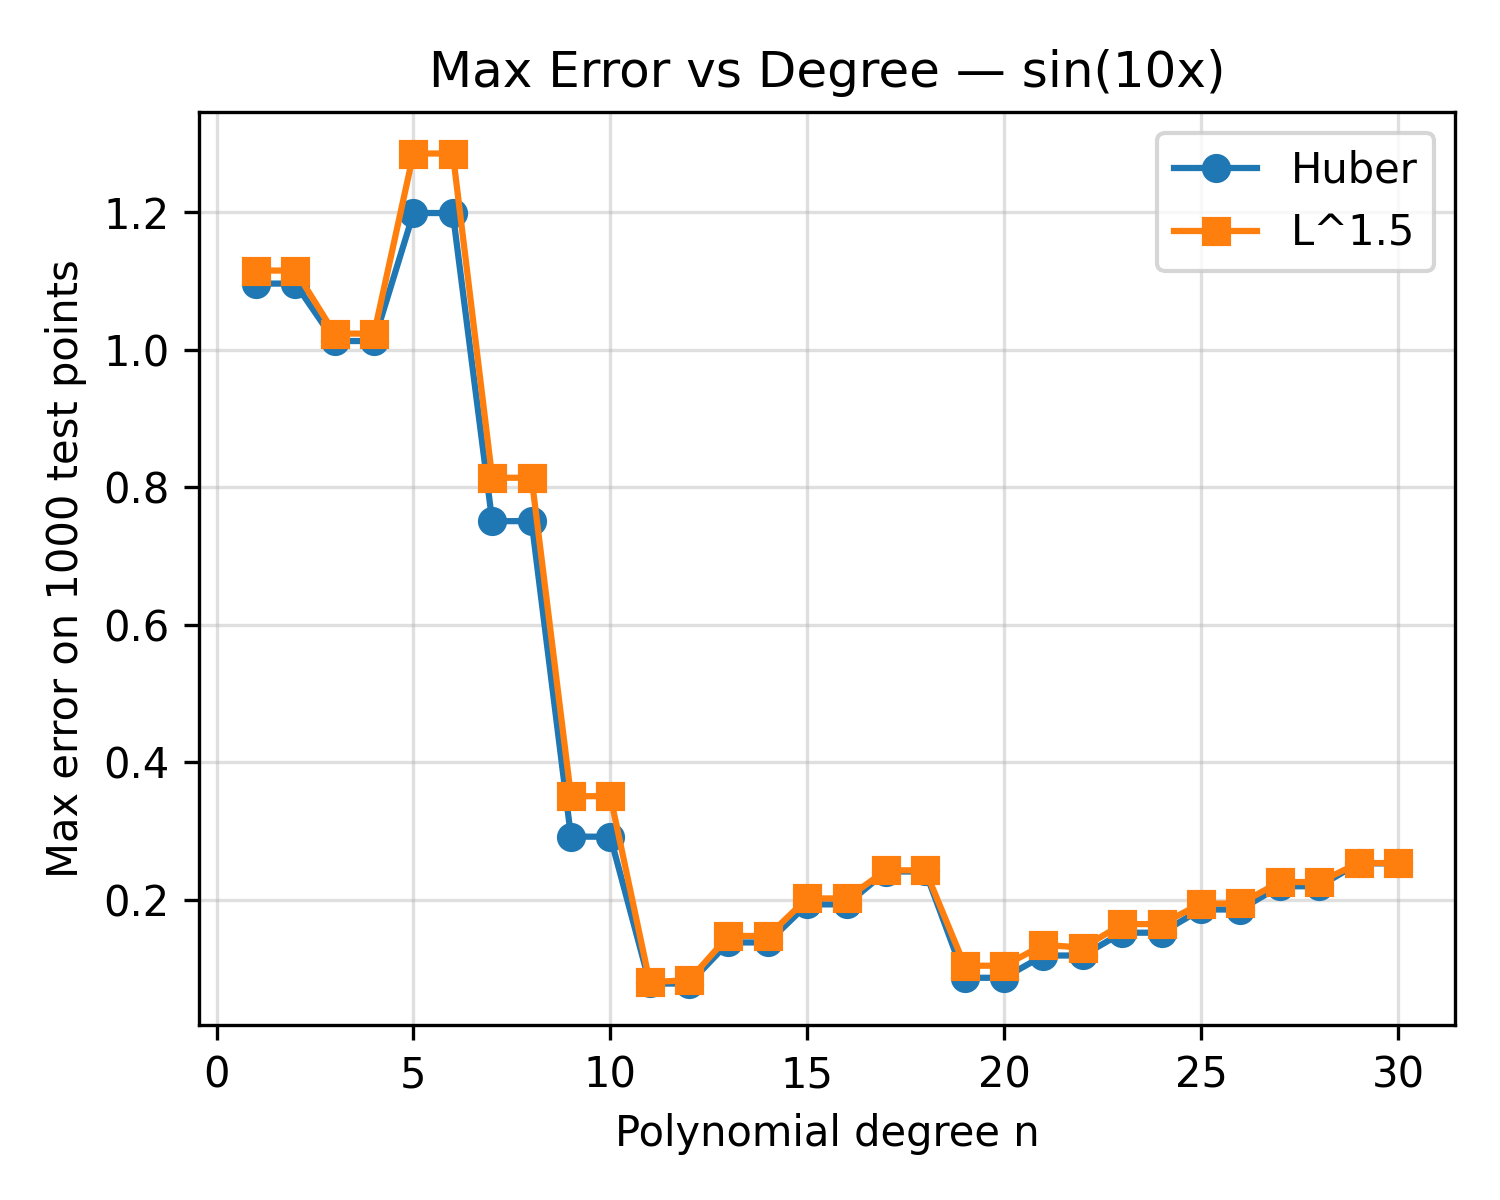
\includegraphics[width=\linewidth]{fig/exercise3_error_vs_degree_sin10x.png}
        %\caption{sin(10x)}
    \end{subfigure}
    \hfill
    \begin{subfigure}[b]{0.49\linewidth}
        \centering
        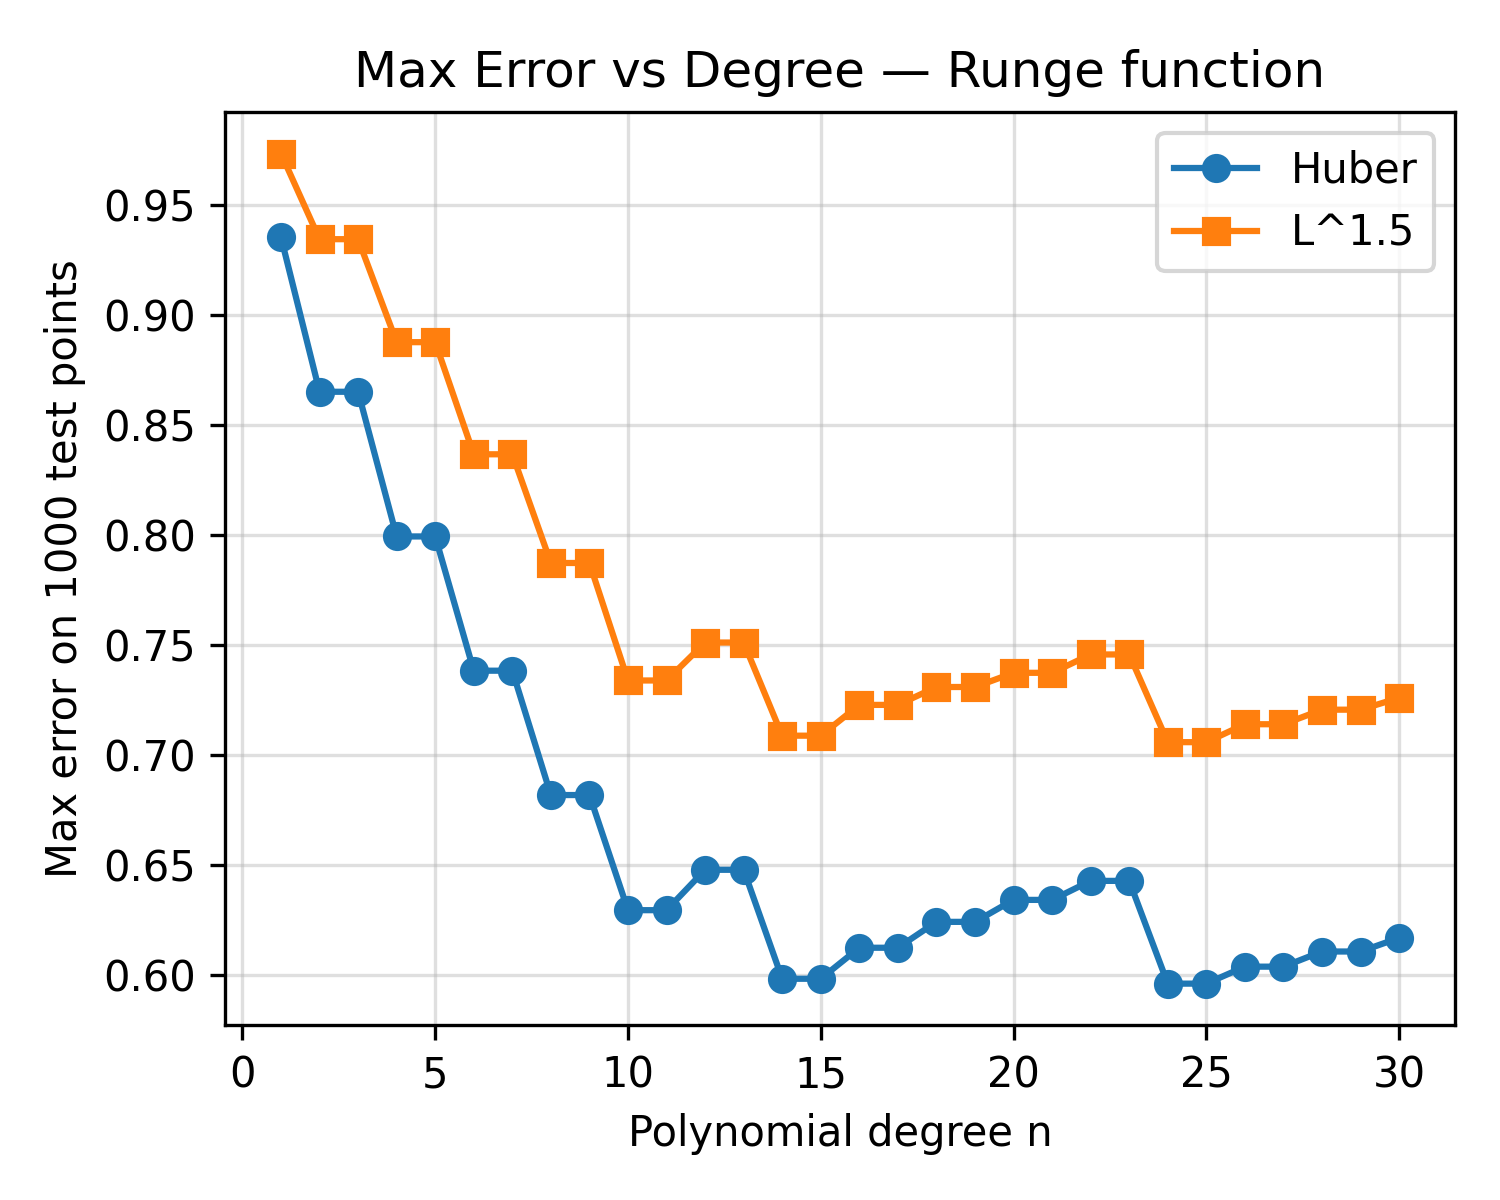
\includegraphics[width=\linewidth]{fig/exercise3_error_vs_degree_Runge_function.png}
        %\caption{Runge function}
    \end{subfigure}
    
    \begin{subfigure}[b]{0.49\linewidth}
        \centering
        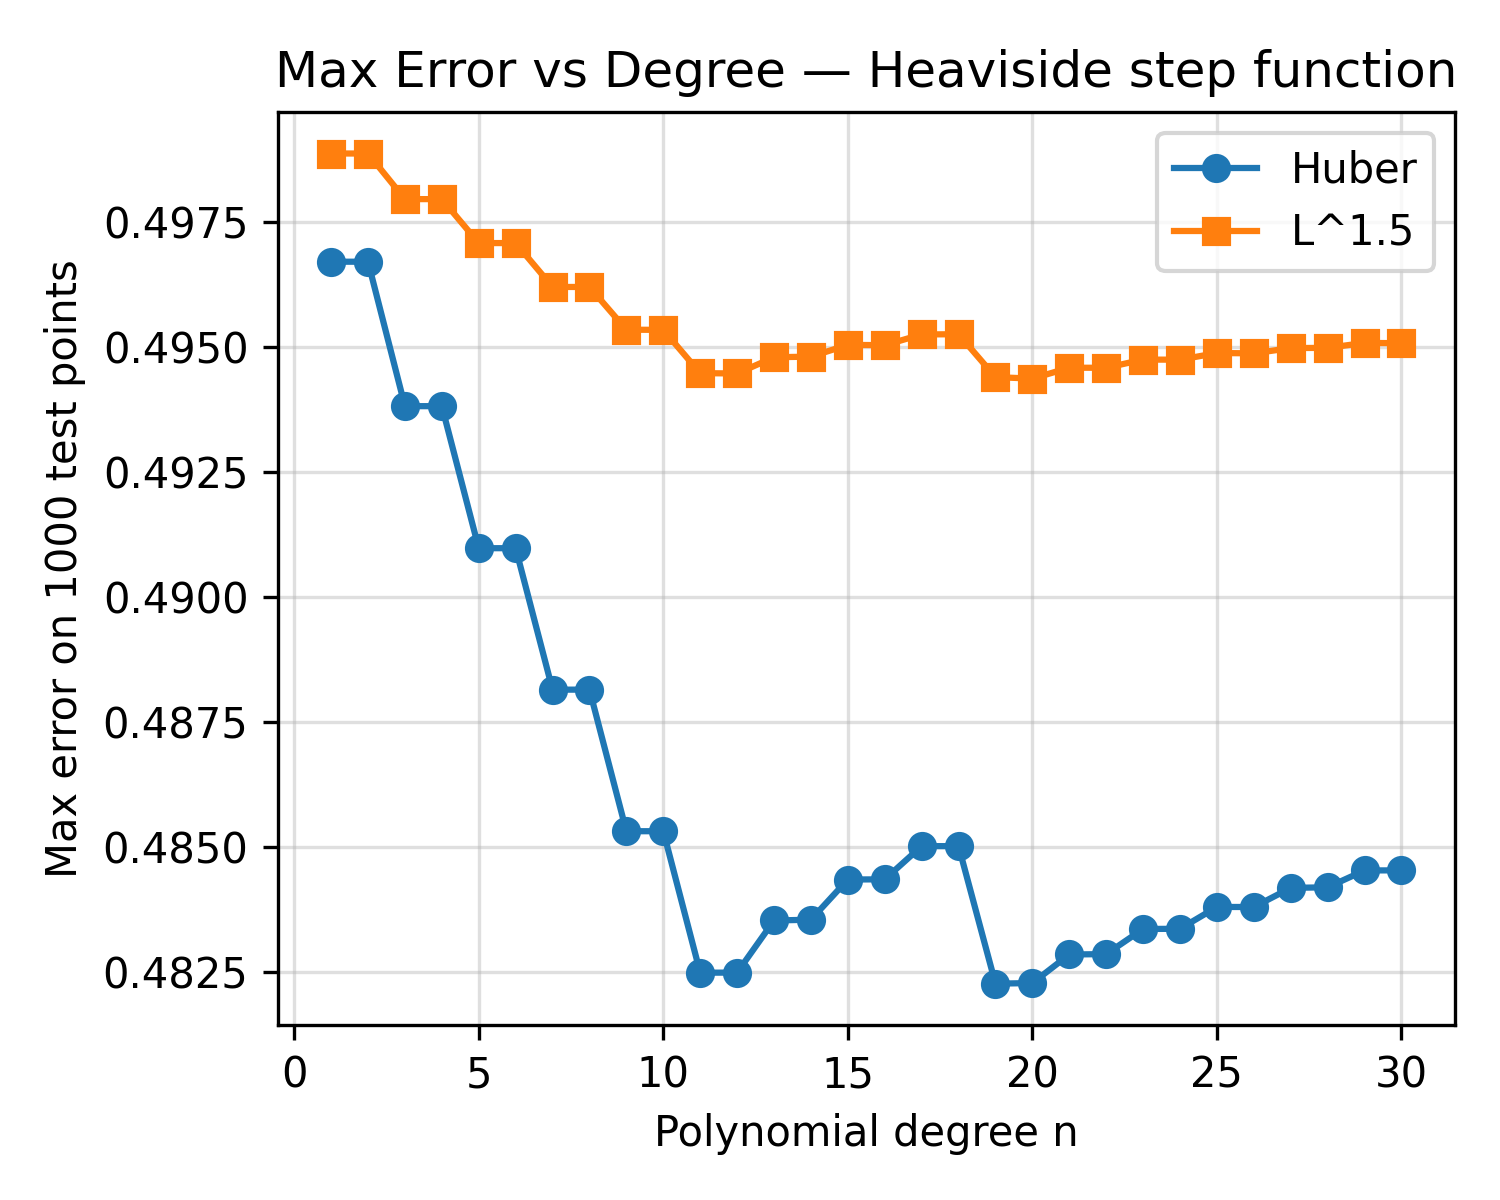
\includegraphics[width=\linewidth]{fig/exercise3_error_vs_degree_Heaviside_step_function.png}
        %\caption{Heaviside step function}
    \end{subfigure}
    
    \caption{Error vs degree for different functions.}
    \label{fig:error-vs-degree}
\end{figure}


\begin{table}[h!]
\centering
\caption{Maximum error $\max_j |\Gamma(x_j) - M(x_j;\theta)|$ 
for selected polynomial degrees $n$ using Huber and $L^{1.5}$ losses.}
\begin{tabular}{llccccc}
\toprule
Dataset & Loss & $n=2$ & $n=5$ & $n=10$ & $n=20$ & $n=30$ \\
\midrule
\multirow{2}{*}{$\sin(10x)$} 
  & Huber        & 1.100 & 1.198 & 0.366 & 0.014 & 0.021 \\
  & $L^{1.5}$    & 1.116 & 1.285 & 0.510 & 0.177 & 0.097 \\
\midrule
\multirow{2}{*}{Runge} 
  & Huber        & 0.868 & 0.802 & 0.632 & 0.580 & 0.569 \\
  & $L^{1.5}$    & 0.938 & 0.891 & 0.737 & 0.689 & 0.675 \\
\midrule
\multirow{2}{*}{Step} 
  & Huber        & 0.499 & 0.497 & 0.496 & 0.495 & 0.495 \\
  & $L^{1.5}$    & 0.499 & 0.498 & 0.497 & 0.495 & 0.495 \\
\bottomrule
\end{tabular}
\label{tab:max-error}
\end{table}

\subsection*{Analysis and Discussion}
The results in \Cref{fig:error-vs-degree} and Table~\ref{tab:max-error} 
show consistent trends across the three datasets. 
For the oscillatory $\sin(10x)$, the $L^{1.5}$ loss initially performs worse (error $0.510$ at 
$n=10$ versus $0.366$ for Huber), but catches up at higher degrees, where 
both methods achieve errors below $0.1$. 
For the Runge function, both losses reduce the maximum error steadily with polynomial 
degree, converging to values below $0.6$ at $n=30$. Although the Runge function $f(x)=1/(1+25x^2)$ is smooth, it is notoriously difficult to approximate with high-degree polynomials on equispaced points. This classical issue, known as Runge's phenomenon, explains why the maximum error decreases only modestly in Table~\ref{tab:max-error}, even as the degree $n$ increases to 30.
In contrast, the discontinuous step function remains difficult: errors plateau around $0.495$, showing that polynomials cannot approximate jumps well. Between the two losses, Huber 
is slightly more stable on the step function, while $L^{1.5}$ shows modest  advantages on oscillatory data at high degrees. Overall, robust losses  provide little benefit on smooth data, some improvement for oscillatory data, and more stability for discontinuities.


%For the three datasets, the results show clear differences in how the Huber and $L^{1.5}$ 
%losses affect polynomial regression. 
%\newpage
%\begin{itemize}
   % \item \textbf{Smooth function (Runge):} Both Huber and $L^{1.5}$ perform well as the polynomial degree increases, with errors decreasing rapidly. Since the data is noise-free and continuous, robust losses offer little advantage over the standard squared error, and both methods converge to similar accuracy. 
    
  %  \item \textbf{Oscillatory function ($\sin(10x)$):} The fits are more sensitive to the choice of loss. As the degree increases, the $L^{1.5}$ loss tends to give slightly smaller maximum errors compared to Huber, suggesting that the heavier weighting of moderate residuals in $L^{1.5}$ better handles the oscillatory structure without amplifying outliers. 
    
  %  \item \textbf{Discontinuous function (Heaviside step):} Both methods struggle, as expected, because polynomials cannot approximate jumps well (Gibbs phenomenon). However, robust losses help reduce the influence of large residuals near the discontinuity. Between the two, Huber usually gives a more balanced fit, while $L^{1.5}$ can emphasize sharper transitions but may introduce oscillations.
%\end{itemize}

%\textbf{Overall conclusion:} For smooth problems, robust losses make little difference, but for oscillatory or discontinuous data, Huber and $L^{1.5}$ can slightly improve stability and reduce worst-case errors. In practice, Huber is often the safer choice for discontinuities, while $L^{1.5}$ may perform better on highly oscillatory signals.

\end{document}